\graphicspath{{chapter_faces/}}
\chapter{Large Pose 3D Face Reconstruction via Volumetric Regression}
\label{chapter:face}

\begin{figure}
  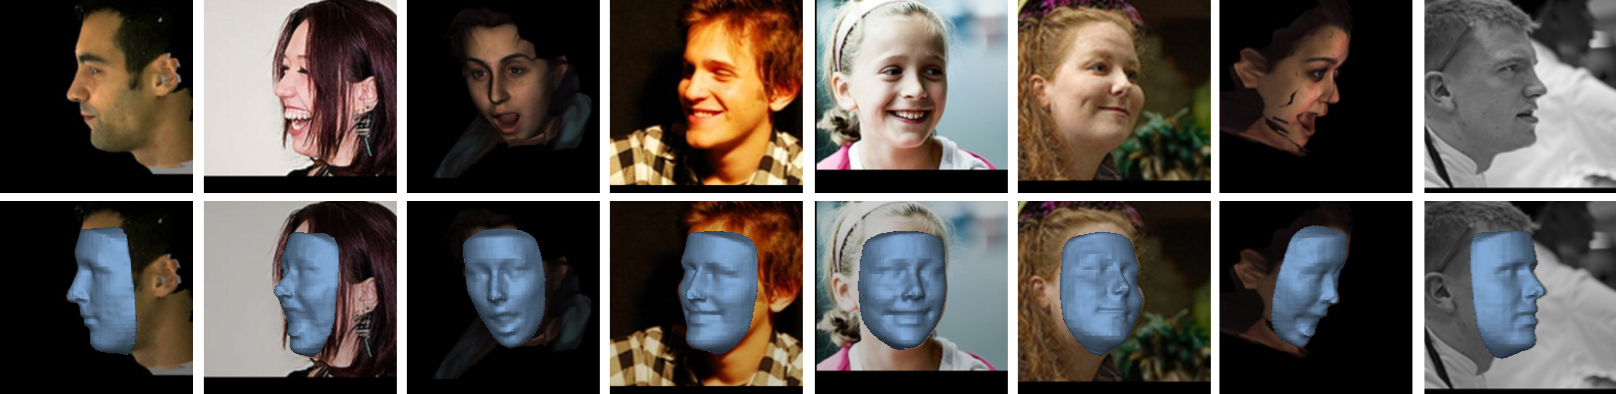
\includegraphics[width=\linewidth]{img/preview.png}
  \caption[A 3D Reconstruction Preview]{A preview of our 3D
    reconstruction method, applied on a wide variety of poses.}
  \label{c:face:fig:preview}
\end{figure}
% \begin{abstract}
%   3D face reconstruction is a fundamental Computer Vision problem of
%   extraordinary difficulty. Current systems often assume the
%   availability of multiple facial images (sometimes from the same
%   subject) as input, and must address a number of methodological
%   challenges such as establishing dense correspondences across large
%   facial poses, expressions, and non-uniform illumination. In general
%   these methods require complex and inefficient pipelines for model
%   building and fitting. In this work, we propose to address many of
%   these limitations by training a Convolutional Neural Network (CNN)
%   on an appropriate dataset consisting of 2D images and 3D facial
%   models or scans. Our CNN works with just a single 2D facial image,
%   does not require accurate alignment nor establishes dense
%   correspondence between images, works for arbitrary facial poses and
%   expressions, and can be used to reconstruct the whole 3D facial
%   geometry (including the non-visible parts of the face) bypassing the
%   construction (during training) and fitting (during testing) of a 3D
%   Morphable Model. We achieve this via a simple CNN architecture that
%   performs direct regression of a volumetric representation of the 3D
%   facial geometry from a single 2D image. We also demonstrate how the
%   related task of facial landmark localization can be incorporated
%   into the proposed framework and help improve reconstruction quality,
%   especially for the cases of large poses and facial
%   expressions. Code and models will be made available at \verb|http://aaronsplace.co.uk|
% \end{abstract}
% \vspace{-4mm}

3D face reconstruction is a fundamental Computer Vision problem, often
considered to be of extraordinary difficultly. Current systems often
assume the availability of multiple facial images as input, sometimes
from the same subject. Additional, there are a number of
methodological challenges involved, which must be addressed. These
challenges include establishing a dense correspondence across large
poses, expressions and non-uniform illumination. In general, these
methods require complex and inefficient pipelines for model building
and fitting. In this work, we propose to address many of these
limitations by constraining the problem of 3D face reconstruction to
the spatial domain. We do this by training a Convolutional Neural
Network (CNN), on an appropriate dataset, consisting of 2D images and
3D facial models, or scans. Our CNN works with just a single 2D facial
image and does not require accurate alignment. Our method works for
arbitrary facial poses and expressions, and can be used to
reconstruction the whole 3D facial geometry, including non-visible
parts. Our method bypasses the construction (during training) and
fitting (during inference) of a 3D Morphable Model. We achieve this via
a simple CNN architecture that performs direct regression of a
volumetric representation of the 3D facial geometry from a single 2D
image. We also demonstrate how the related task of facial landmark
localisation can be incorporated into the proposed framework and help
improve reconstruction quality, especially in the cases of large poses
and facial expressions.


\section{Introduction}
3D face reconstruction is the problem of recovering the 3D facial
geometry from 2D images. Despite many years of research, it is still
an open problem in Computer Vision and Graphics research. Depending on
the setting and the assumptions made, there are many variations of it,
as well as a multitude of approaches to solve it. This work is on 3D
face reconstruction using only a single image. Under this setting, the
problem is considered far from being solved. In this chapter, we
propose to approach it, for the first time to the best of our
knowledge, by directly learning a mapping from pixels to 3D
coordinates using a Convolutional Neural Network (CNN). Besides its
simplicity, our approach works with totally unconstrained images
downloaded from the web, including facial images of arbitrary poses,
facial expressions and occlusions, as shown in
Figure~\ref{c:face:fig:preview}. \newline \textbf{Motivation.} No
matter what the underlying assumptions are, what the input(s) and
output(s) to the algorithm are, 3D face reconstruction requires in
general complex pipelines and solving non-convex difficult
optimization problems for both model building (during training) and
model fitting (during testing). In the following paragraphs, we provide
examples from 5 predominant approaches:

\begin{enumerate}
\item In the 3D Morphable Model (3DMM) \cite{blanz1999morphable,
    romdhani2005estimating}, the most popular approach for estimating
  the full 3D facial structure from a single image (among others),
  training includes an iterative flow procedure for dense image
  correspondence which is prone to failure. Additionally, testing
  requires a careful initialisation for solving a difficult highly
  non-convex optimization problem in order to estimate the pose and
  shape parameters, which is slow.
\item The work of \cite{kemelmacher20113d}, a popular approach for
  2.5D reconstruction from a single image, formulates and solves a
  carefully initialised (for frontal images only) non-convex
  optimization problem for recovering the lighting, depth, and albedo
  in an alternating manner where each of the sub-problems is a
  difficult optimization problem per se.
\item In \cite{kemelmacher2011face}, a quite popular recent approach
  for creating a neutral subject-specific 2.5D model from a near
  frontal image, an iterative procedure is proposed which entails
  localising facial landmarks, face frontalization, solving a
  photometric stereo problem, local surface normal estimation, and
  finally shape integration.
\item In \cite{suwajanakorn2014total}, a state-of-the-art pipeline for
  reconstructing a highly detailed 2.5D facial shape for each video
  frame, an average shape and an illumination subspace for the
  specific person is firstly computed (offline), while testing is an
  iterative process requiring a sophisticated pose estimation
  algorithm, 3D flow computation between the model and the video
  frame, and finally shape refinement by solving a shape-from-shading
  optimization problem.
\item More recently, the state-of-the-art method of
  \cite{roth2016adaptive} that produces the average (neutral) 3D face
  from a collection of personal photos, firstly performs landmark
  detection, then fits a 3DMM using a sparse set of points, then
  solves an optimization problem similar to the one in
  \cite{kemelmacher2011face}, then performs surface normal estimation
  as in \cite{kemelmacher2011face} and finally performs surface
  reconstruction by solving another energy minimisation problem.
\end{enumerate}

Simplifying the technical challenges involved in the aforementioned
works is the main motivation of this work.

\subsection{Main contributions}
We describe a very simple approach which bypasses many of the
difficulties encountered in 3D face reconstruction by using a
novel volumetric representation of the 3D facial geometry, and
an appropriate CNN architecture that is trained to regress directly
from a 2D facial image to the corresponding 3D volume. An overview of
our method is shown in Figure~\ref{fig:cnnall}. In summary, our contributions
are:
\begin{itemize}
\item Given a dataset consisting of 2D images and 3D face scans, we
  investigate whether a CNN can learn directly, in an end-to-end
  fashion, the mapping from image pixels to the full 3D facial
  structure geometry (including the non-visible facial parts). Indeed,
  we show that the answer to this question is positive.
\item We demonstrate that our CNN works with just a single 2D facial
  image, does not require accurate alignment nor establishes dense
  correspondence between images, works for arbitrary facial poses and
  expressions, and can be used to reconstruct the whole 3D facial
  geometry bypassing the construction (during training) and fitting
  (during testing) of a 3DMM.
\item We achieve this via a simple CNN architecture that performs
  \textit{direct} regression of a volumetric representation of the 3D
  facial geometry from a single 2D image. 3DMM fitting is not
  used. Our method uses only 2D images as input to the proposed CNN
  architecture.
\item We show how the related task of 3D facial landmark localisation
  can be incorporated into the proposed framework and help improve
  reconstruction quality, especially for the cases of large poses and
  facial expressions.
\item We report results for a large number of experiments on both
  controlled and completely unconstrained images from the web,
  illustrating that our method outperforms prior work on single image
  3D face reconstruction by a large margin.
\end{itemize}

\section{Method}


This section describes our framework including the proposed data representation used.


\subsection{Dataset}

Our aim is to regress the full 3D facial structure from a 2D image. To
this end, our method requires an appropriate dataset consisting of 2D
images and 3D facial scans. As our target is to apply the method on
completely unconstrained images from the web, we chose the dataset of
\cite{zhu2016face} for forming our training and test sets. The dataset
has been produced by fitting a 3DMM built from the combination of the
Basel \cite{paysan20093d} and FaceWarehouse
\cite{cao2014facewarehouse} models to the unconstrained images of the
300W dataset \cite{sagonas2013semi} using the multi-feature fitting
approach of \cite{romdhani2005estimating}, careful initialisation and
by constraining the solution using a sparse set of landmarks. Face
profiling is then used to render each image to 10-15 different poses
resulting in a large scale dataset (more than 60,000 2D facial images
and 3D meshes) called 300W-LP. Each mesh consists of approximately
53000 vertices, enclosing the face entirely. However, no vertices
exist around the mouth, base of neck and eyes, and as such, this mesh
is not watertight. All images are $450 \times 450$, although these are
downsampled to $386 \times 386$ during training. Note that because
each mesh is produced by a 3DMM, the vertices of all produced meshes
are in dense correspondence; however this is not a prerequisite for
our method and unregistered raw facial scans could be also used if
available (e.g. the BU-4DFE dataset~\cite{yin2008high}).

\subsection{Proposed volumetric representation}

Our goal is to predict the coordinates of the 3D vertices of each
facial scan from the corresponding 2D image via CNN regression. As a
number of works have pointed out (see for example
\cite{tompson2015efficient, pfister2015flowing}), direct regression of
all 3D points concatenated as a vector using the standard L2 loss
might cause difficulties in learning because a single correct value
for each 3D vertex must be predicted. Additionally, such an approach
requires interpolating all scans to a vector of a fixed dimension, a
pre-processing step not required by our method. Note that similar
learning problems are encountered when a CNN is used to regress model
parameters like the 3DMM parameters rather than the actual
vertices. In this case, special care must be taken to weight
parameters appropriately using the Mahalanobis distance or in general
some normalisation method, see for example \cite{zhu2016face}. We
compare the performance of our method with that of a similar
method~\cite{zhu2016face} in Section~\ref{S:Results}.

\begin{figure}
  \centering
  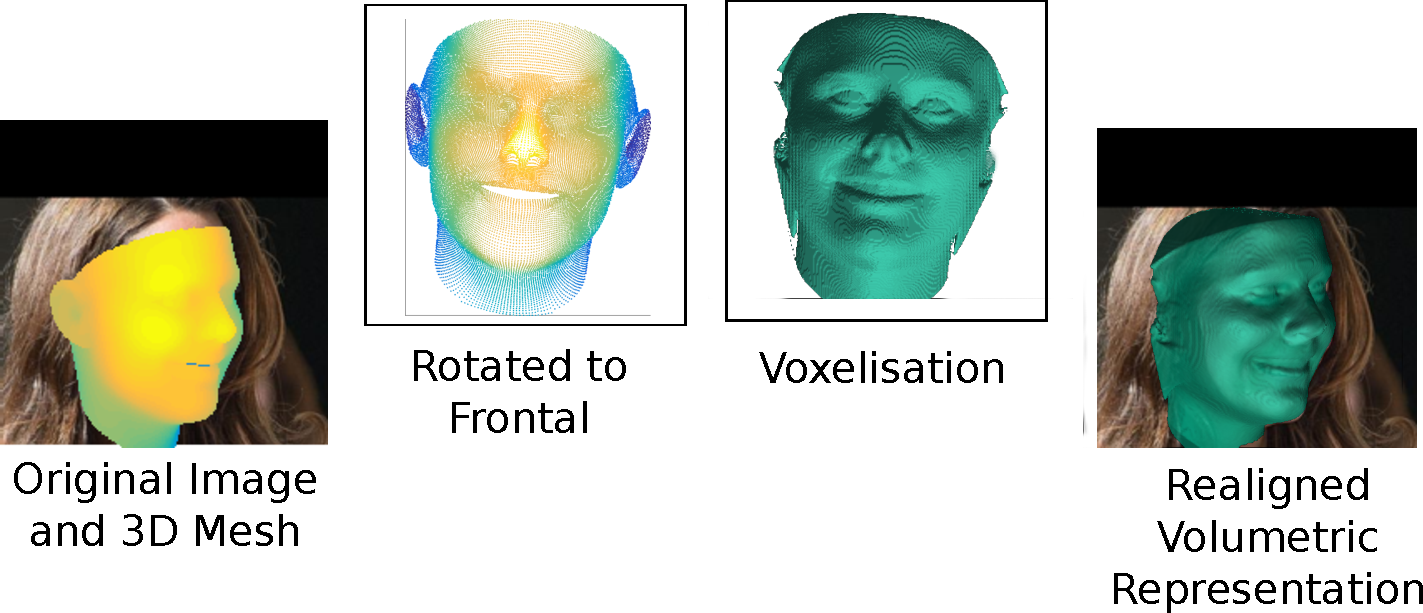
\includegraphics[width=0.9\linewidth]{img/discretisation.pdf}

  \caption[Dataset voxelisation procedure]{The voxelisation process
    creates a volumetric representation of the 3D face mesh, aligned
    with the 2D image.}
  \label{fig:discretisation}
\end{figure}

% Is it reasonable to say 2D to 3D image segmentation?
To alleviate the aforementioned learning problem, we propose to
reformulate the problem of 3D face reconstruction as one of 2D to 3D
image segmentation: in particular, we convert each 3D facial scan into
a 3D binary volume $\mathbf{V}_{whd}$ by discretizing the 3D space
into voxels $\{w,h,d\}$, assigning a value of 1 to all points enclosed
by the 3D facial scan, and 0 otherwise. That is to say $ V_{whd}$ is
the ground truth for voxel $\{w,h,d\}$ and is equal to 1, if voxel
$\{w,h,d\}$ belongs to the 3D volumetric representation of the face
and 0 otherwise (i.e. it belongs to the background). The conversion is
shown in Figure~\ref{fig:discretisation}. Contrary to standard
approaches, this data was voxelised by rotating to frontal and
estimating a depth map is estimated using bilinear interpolation. from
which the volume is filled back to a fixed point. This results in the
mouth becoming filled. Notice that the process creates a volume fully
aligned with the 2D image. The importance of spatial alignment is
analysed in more detail in Section~\ref{sec:spatialimportance}. The
error caused by discretization for a randomly picked facial scan as a
function of the volume size is shown in
Figure~\ref{fig:voxerror}. Given that the error of state-of-the-art
methods \cite{roth2016adaptive,liu2016joint} is of the order of a few
mms, we conclude that discretization by $192\times 192\times 200$
produces negligible error. Such a spatial resolution is ideal for the
type of architecture we have chosen to use as it can be reduced by
half many times. The depth, 200, was chosen to capture as much depth
information as possible without sacrificing the spatial resolution or
increasing the memory requirements too much.

Given our volumetric facial representation, the problem of regressing
the 3D coordinates of all vertices of a facial scan is reduced to one
of 3D binary volume segmentation. We approach this problem using
recent CNN architectures from semantic image segmentation
\cite{long2015fully} and their extensions \cite{newell2016stacked}, as
described in the next subsection.

\begin{figure}
  \centering
  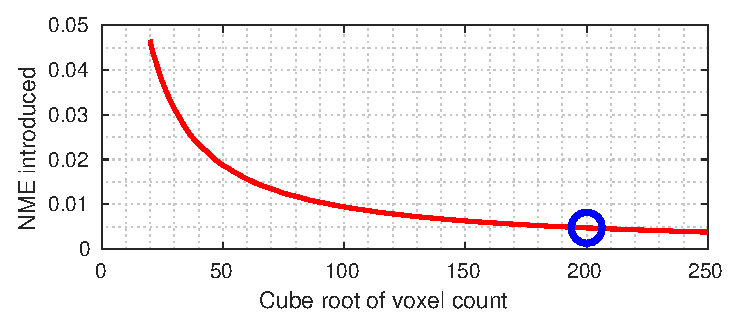
\includegraphics[width=0.9\linewidth]{curves/voxerror.eps}
  \caption[Error due to voxelisation]{The error introduced due to
    voxelisation, shown as a function of volume density.}
  \label{fig:voxerror}
\end{figure}

\subsection{Volumetric Regression Networks}


In this section, we describe the proposed volumetric regression
network, exploring several architectural variations described in
detail in the following subsections:

\textbf{Volumetric Regression Network (VRN)}. We wish to learn a
mapping from the 2D facial image to its corresponding 3D volume
$f: \mathbf{I} \rightarrow \mathbf{V}$. Given the training set of 2D
images and constructed volumes, we learn this mapping using a CNN. Our
CNN architecture for 3D segmentation is based on the ``hourglass
network'' of \cite{newell2016stacked} an extension of the fully
convolutional network of \cite{long2015fully} using skip connections
and residual learning \cite{he2015deep}. Our volumetric architecture
consists of two hourglass modules which are stacked together without
intermediate supervision. The input is an RGB image and the output is
a volume of $192\times 192\times 200$ of real values. This
architecture is shown in Figure~\ref{fig:cnnbaseline}. As it can be
observed, the network has an encoding/decoding structure where a set
of convolutional layers are firstly used to compute a feature
representation of fixed dimension. This representation is further
processed back to the spatial domain, re-establishing spatial
correspondence between the input image and the output volume. Features
are hierarchically combined from different resolutions to make
per-pixel predictions. The second hourglass is used to refine this
output, and has an identical structure to that of the first one.

\begin{figure*}
  \centering
  \begin{subfigure}[t]{1\textwidth}
    \centering
    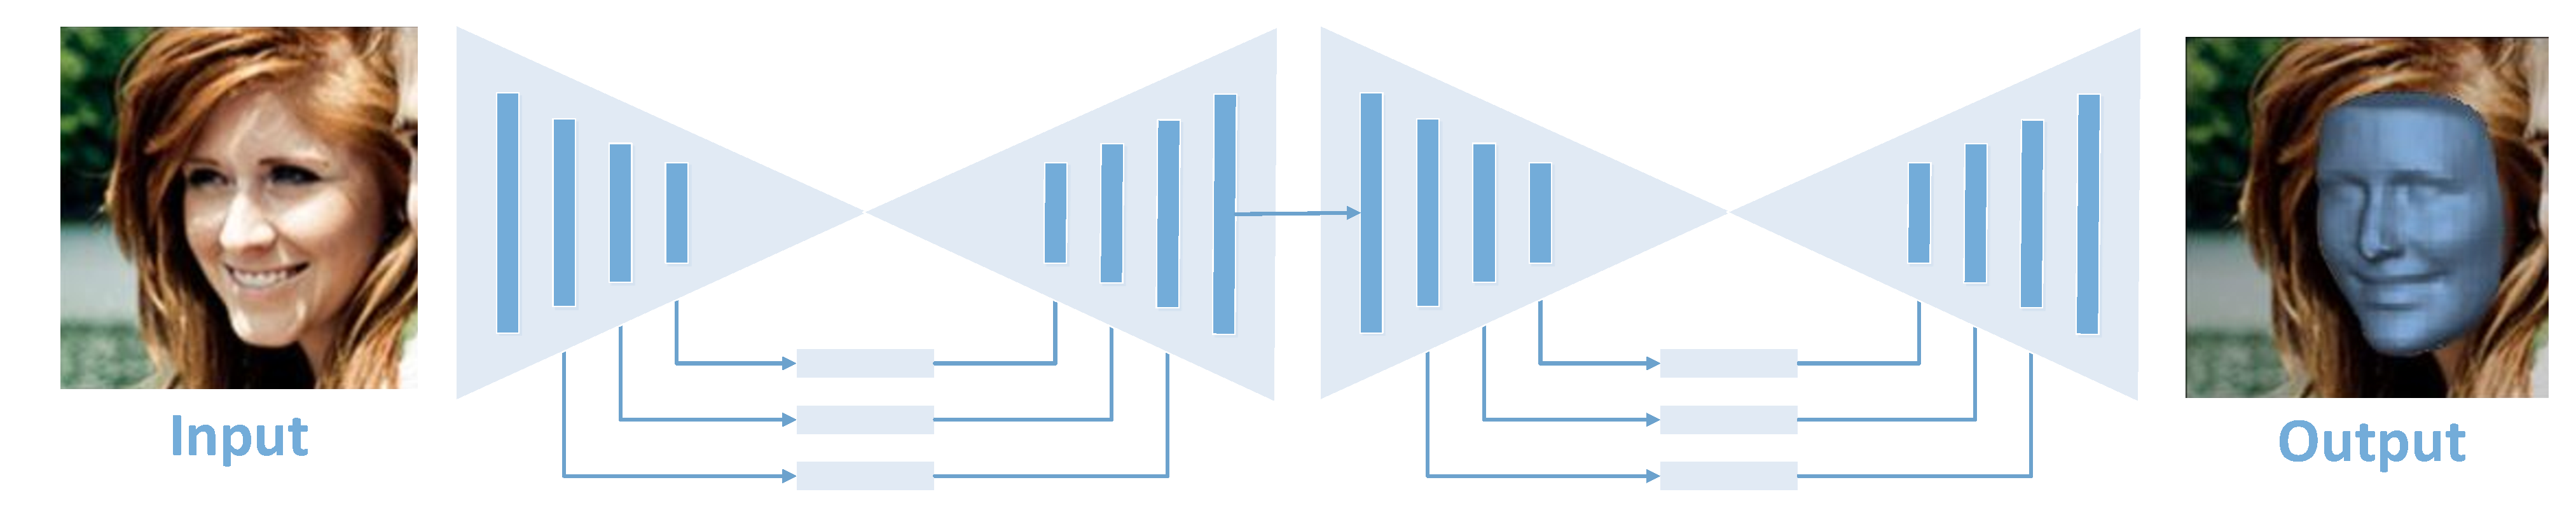
\includegraphics[width=0.81\linewidth]{img/baseline.pdf}
    \caption[Baseline reconstruction architecture]{The proposed
      \textit{Volumetric Regression Network (VRN)} accepts as input an
      RGB input and directly regresses a 3D volume completely bypassing
      the fitting of a 3DMM. Each rectangle is a residual module of 256
      features.}

    \label{fig:cnnbaseline}
  \end{subfigure}
  ~
  \begin{subfigure}[t]{1\textwidth}
    \centering
    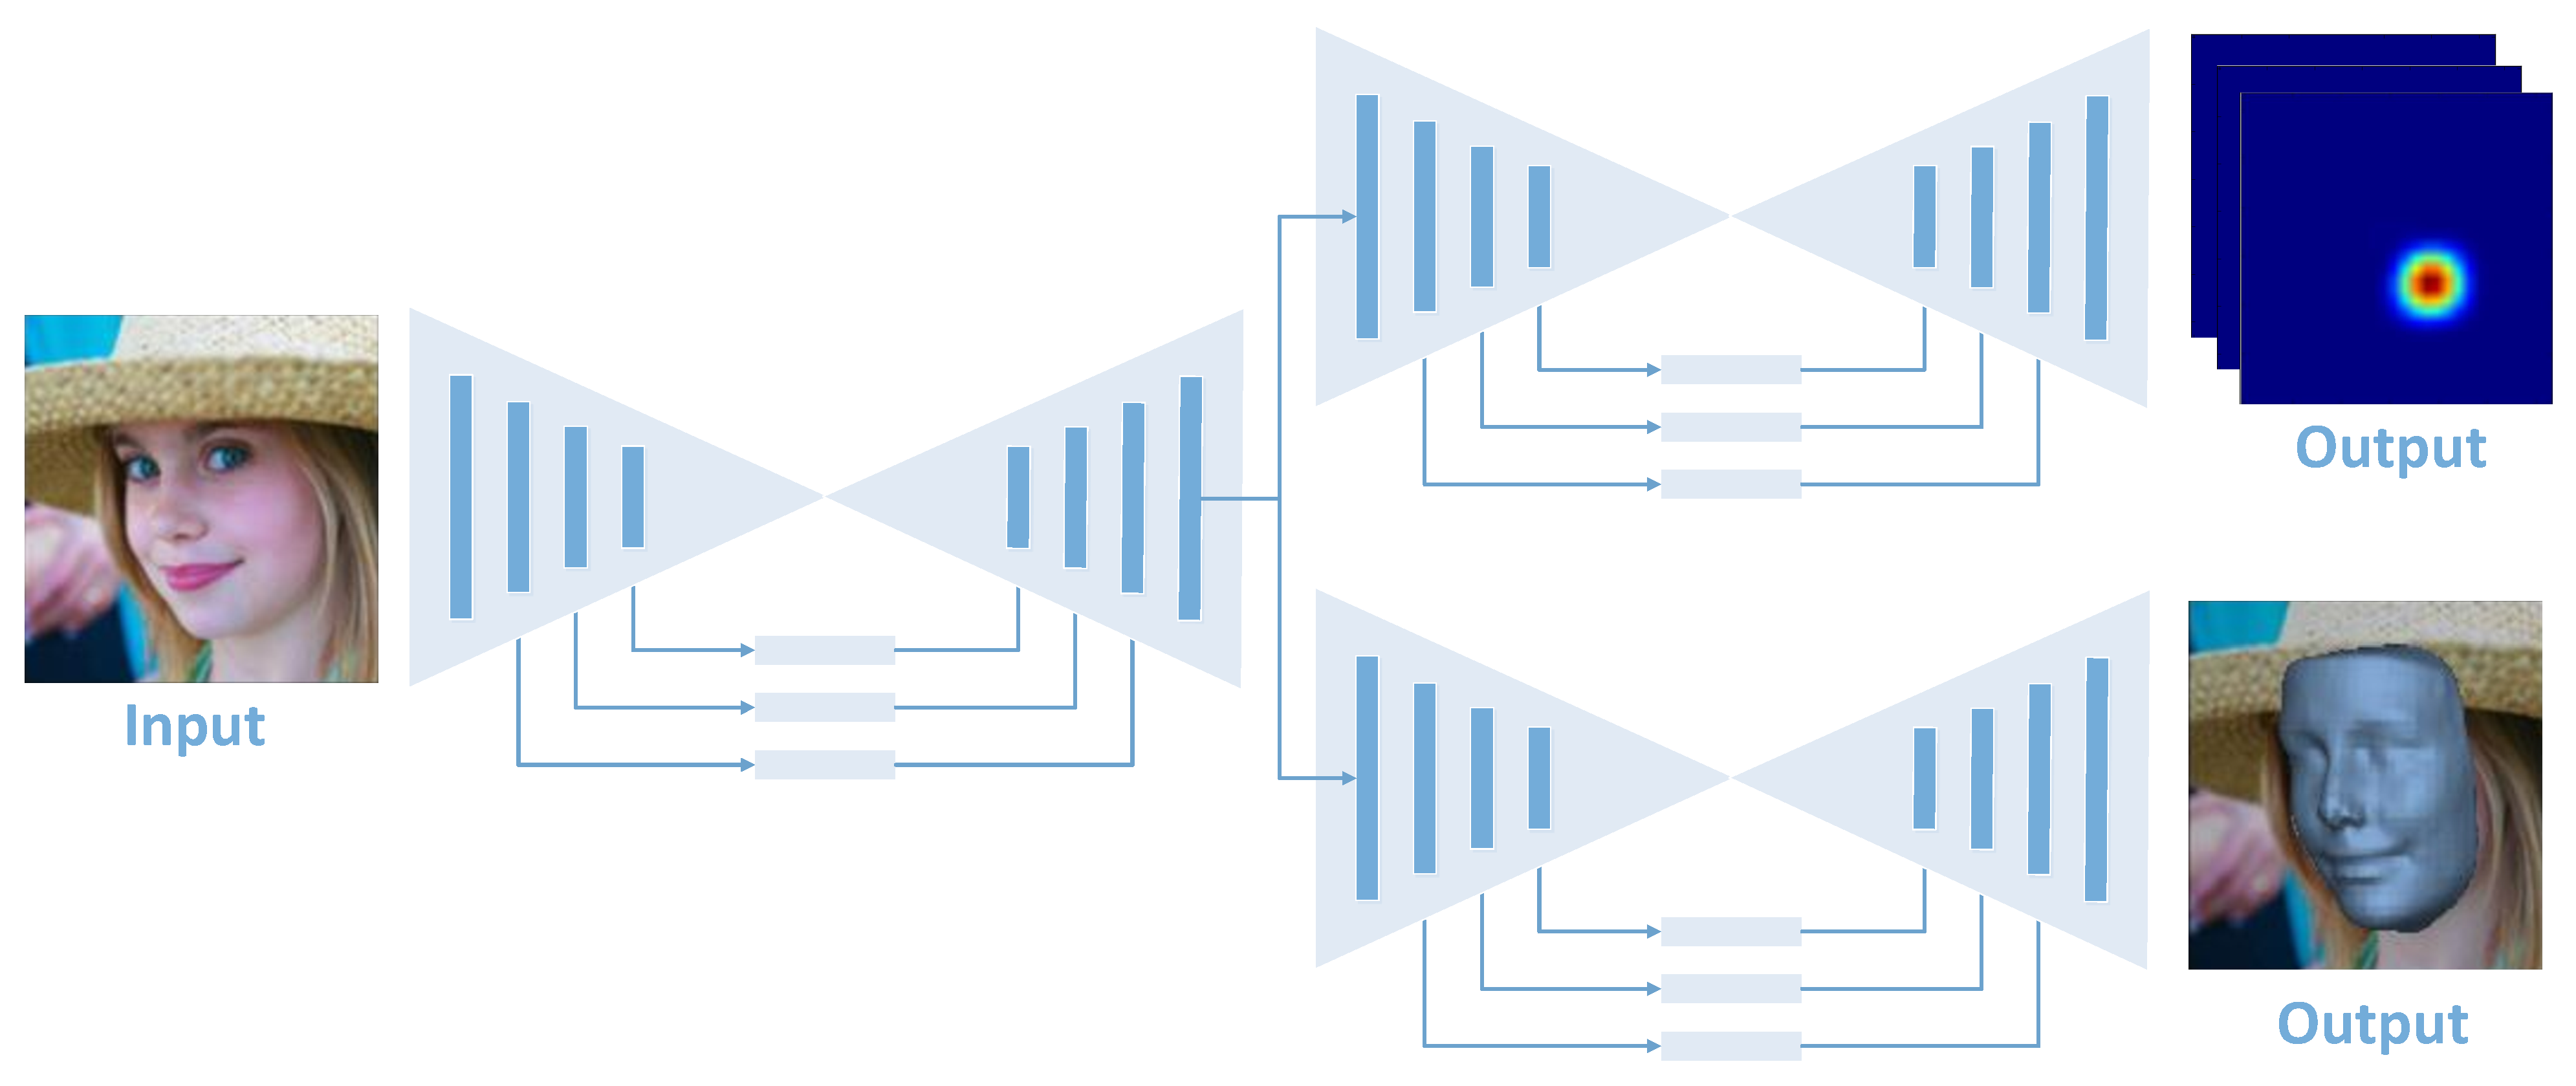
\includegraphics[width=0.6\linewidth]{img/multitask.pdf}
    \caption[Multitask reconstruction architecture]{The proposed
      \textit{VRN - Multitask} architecture regresses both the 3D facial
      volume and a set of sparse facial landmarks.}
    \label{fig:cnnmultitask}
    \vspace{-2mm}
  \end{subfigure}
  ~
  \begin{subfigure}[t]{0.98\textwidth}
    \centering
    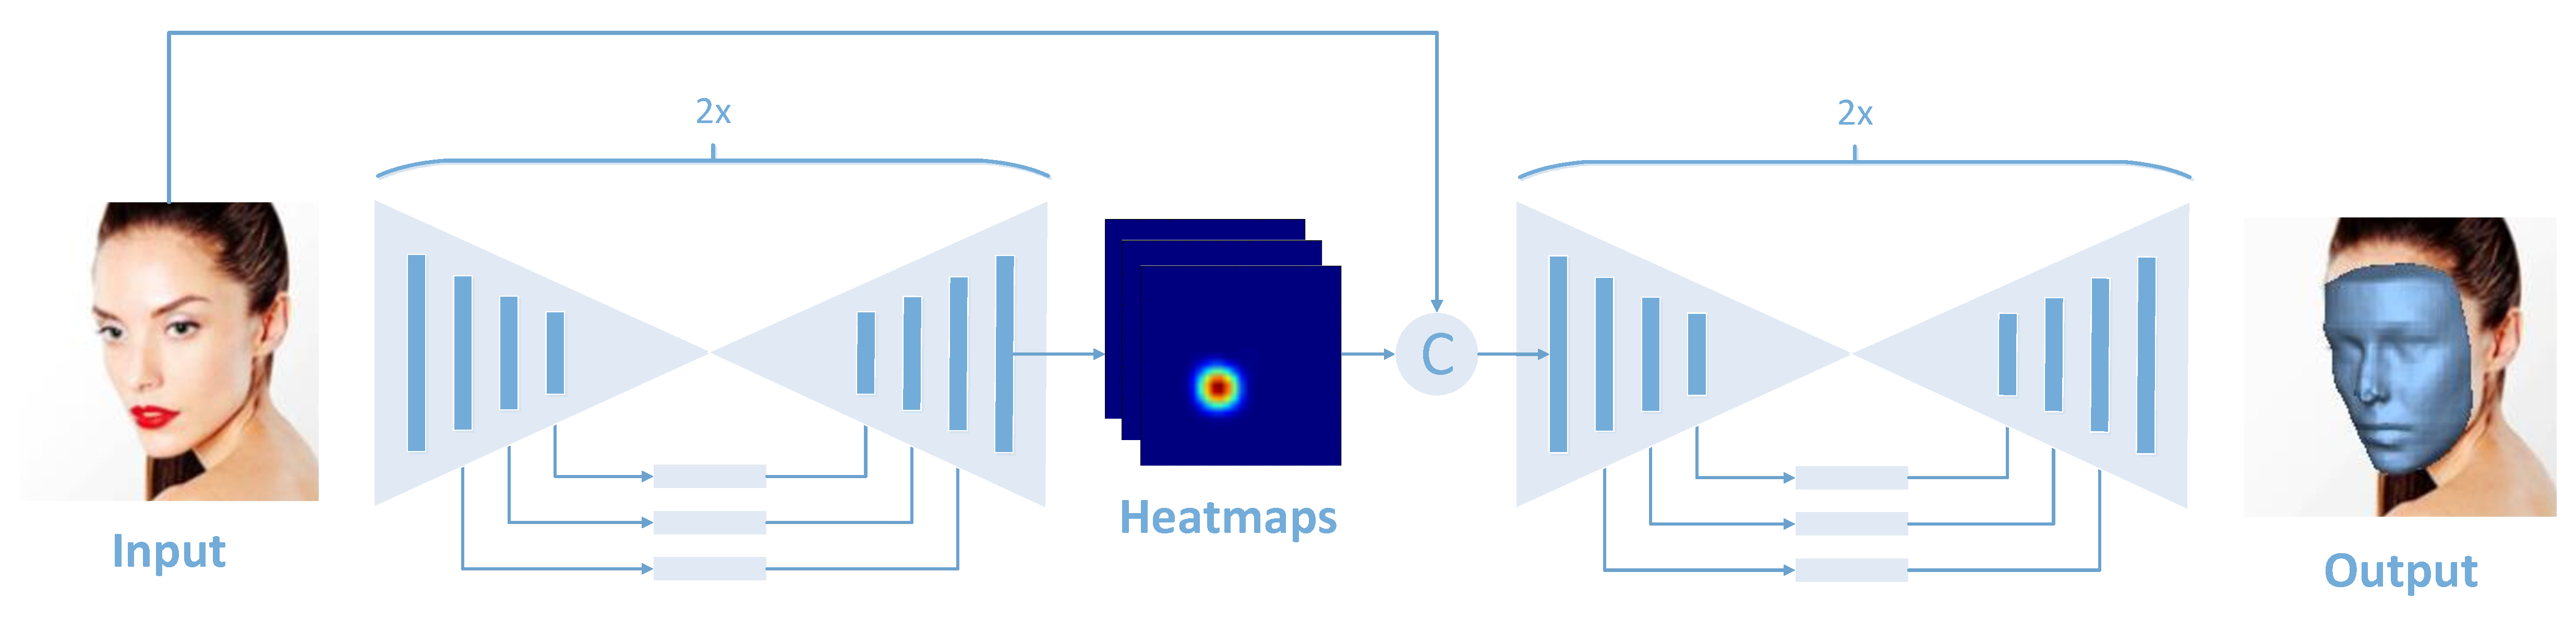
\includegraphics[width=\linewidth]{img/guided.pdf}
    \caption[Guided reconstruction architecture]{The proposed
      \textit{VRN - Guided} architecture firsts detects the 2D
      projection of the 3D landmarks, and stacks these with the original
      image. This stack is fed into the reconstruction network, which
      directly regresses the volume.}
    \label{fig:guidednet}
  \end{subfigure}
  ~
  \caption[Overview of proposed architectures]{An overview of the
    proposed three architectures for Volumetric Regression:
    \textit{Volumetric Regression Network (VRN)}, \textit{VRN -
      Multitask} and \textit{VRN - Guided}.}
  \label{fig:cnnall}
  \vspace{-5mm}
\end{figure*}

We train our volumetric regression network using the sigmoid cross
entropy loss function:
\begin{equation} l_{1} = \sum\limits_{w=1}^{W}
  \sum\limits_{h=1}^{H}\sum\limits_{d=1}^{D}[V_{whd}\log
  \widehat{V}_{whd}+(1-V_{whd})\log(1-\widehat{V}_{whd})],
\end{equation} where $\widehat{V}_{whd}$ is the corresponding Sigmoid
output at voxel $\{w,h,d\}$ of the regressed volume. In the case of
\textit{VRN - Multitask}, the same loss is applied to both tails of
the network with even weightings. Similarly, in \textit{VRN - Guided},
the loss is also applied to the heatmap regression and hence the loss
is summed during backpropagation.

Each residual module of all three of our architectures consists of 256
feature spatial convolutions.

At test time, and given an input 2D image, the network regresses a 3D
volume from which the outer 3D facial mesh is recovered. Rather than
making hard (binary) predictions at pixel level, we found that the
soft sigmoid output is more useful for further processing. Both
representations are shown in Figure~\ref{fig:roughvssmooth} where
clearly the latter results in smoother results. Finally, from the 3D
volume, a mesh can be formed by generating the iso-surface of the
volume. If needed, correspondence between this variable length mesh
and a fixed mesh can be found using Iterative Closest Point (ICP).

\textbf{VRN - Multitask}. We also propose a Multitask VRN, shown in
Figure~\ref{fig:cnnmultitask}, consisting of three hourglass
modules. The first hourglass provides features to a fork of two
hourglasses. The first of this fork regresses the 68 iBUG landmarks
\cite{sagonas2013semi} as 2D Gaussians, each on a separate
channel. The second hourglass of this fork directly regresses the 3D
structure of the face as a volume, as in the aforementioned unguided
volumetric regression method. The goal of this multitask network is to
learn more reliable features which are better suited to the two tasks.


\begin{figure}
  \centering
  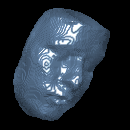
\includegraphics[width=0.2\linewidth]{img/example_rough.png}
  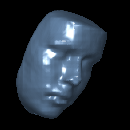
\includegraphics[width=0.2\linewidth]{img/example_smooth.png}
  \caption[Binary vs Real volumes]{Comparison between making hard
    (binary) vs soft (real) predictions. The latter produces a
    smoother result.}
  \label{fig:roughvssmooth}
  \vspace{-4mm}
\end{figure}


\textbf{VRN - Guided}. We argue that reconstruction should benefit
from firstly performing a simpler face analysis task; in particular we
propose an architecture for volumetric regression guided by facial
landmarks. To this end, we train a stacked hourglass network which
accepts guidance from landmarks during training and inference. This
network has a similar architecture to the unguided volumetric
regression method, however the input to this architecture is an RGB
image stacked with 68 channels, each containing a Gaussian ($\sigma =
1$, approximate diameter of 6 pixels) centred on each of the 68
landmarks. This stacked representation and architecture is
demonstrated in Figure~\ref{fig:guidednet}. During training we used the
ground truth landmarks while during testing we used a stacked
hourglass network trained for facial landmark localisation. We call
this network \textit{VRN - Guided}.




\subsection{Training}

% Trained with RMSProp
Each of our architectures was trained end-to-end using RMSProp with an
initial learning rate of $10^{-4}$, which was lowered after 40 epochs
to $10^{-5}$. This training protocol remained fixed for all
architectures to avoid bias. The number of epochs were chosen based on
the rate at which the learning rate fell during training of
\textit{VRN} and some tests using the testing set of the
HELEN~\cite{le2012interactive} images from
300W~\cite{sagonas2013semi} as validation. During training,
random augmentation was applied to each input sample (face image) and
its corresponding target (3D volume): we applied in-plane rotation
$r\in[-45^{\circ}, ..., 45^{\circ}]$, translation
$t_z,t_y\in[-15,...,15]$ and scale $s\in [0.85,...,1.15]$ jitter. In
20\% of cases, the input and target were flipped
horizontally. Finally, the input samples were adjusted with some
colour scaling on each RGB channel selected uniformly
$c_r,c_g,c_b \in \{0.6,...,1.4\}$.

In the case of the \textit{VRN - Guided}, the landmark detection
module was trained to regress Gaussians with standard deviation of
approximately 3 pixels ($\sigma = 1$). We noticed near negligible
reduction in 3D reconstruction performance when training with
different standard deviations.

% dataset selection

% Gaussian size (sigma 1)
% Learning rate

\section{Results} \label{S:Results}

\subsection{Evaluation Datasets}

We used three different datasets for quantifying the performance of
our method. The dataset AFLW2000-3D allows for unbiased and fair
comparison with other methods. The remaining two, BU-4DFE and
Florence, have to be rendered, but allows us to quantify performance
across pose and expression with greater accuracy. These three datasets
are discussed in more detail below.

\paragraph{(a) AFLW2000-3D} As our target was to test
our network on totally unconstrained images, we firstly conducted
experiments on the AFLW2000-3D~\cite{zhu2016face} dataset which
contains 3D facial meshes for the first 2000 images from AFLW
\cite{aflw2011}.

\paragraph{(b) BU-4DFE} We also conducted experiments on rendered
images from BU-4DFE~\cite{yin2008high}. We rendered each participant
for both Happy and Surprised expressions with three different pitch
rotations between $-20$ and $20$ degrees. For each pitch, seven roll
rotations from $-80$ to $80$ degrees were also rendered. Large
variations in lighting direction and colour were added randomly to
make the images more challenging. We show some example renderings in
the first row (a) of Figure~\ref{fig:example_renderings}.

\paragraph{(c) Florence}
Finally, we conducted experiments on rendered images from the
Florence~\cite{masi2d3dFaceData} dataset. Facial images were rendered
in a similar fashion to the ones of BU-4DFE but for slightly different
parameters: Each face is rendered in 20 difference poses, using a
pitch of -15, 20 or 25 degrees and each of the five evenly spaced
rotations between -80 and 80. We show some example renderings in the
second (b) row of Figure~\ref{fig:example_renderings}.

\begin{figure}
  \centering
  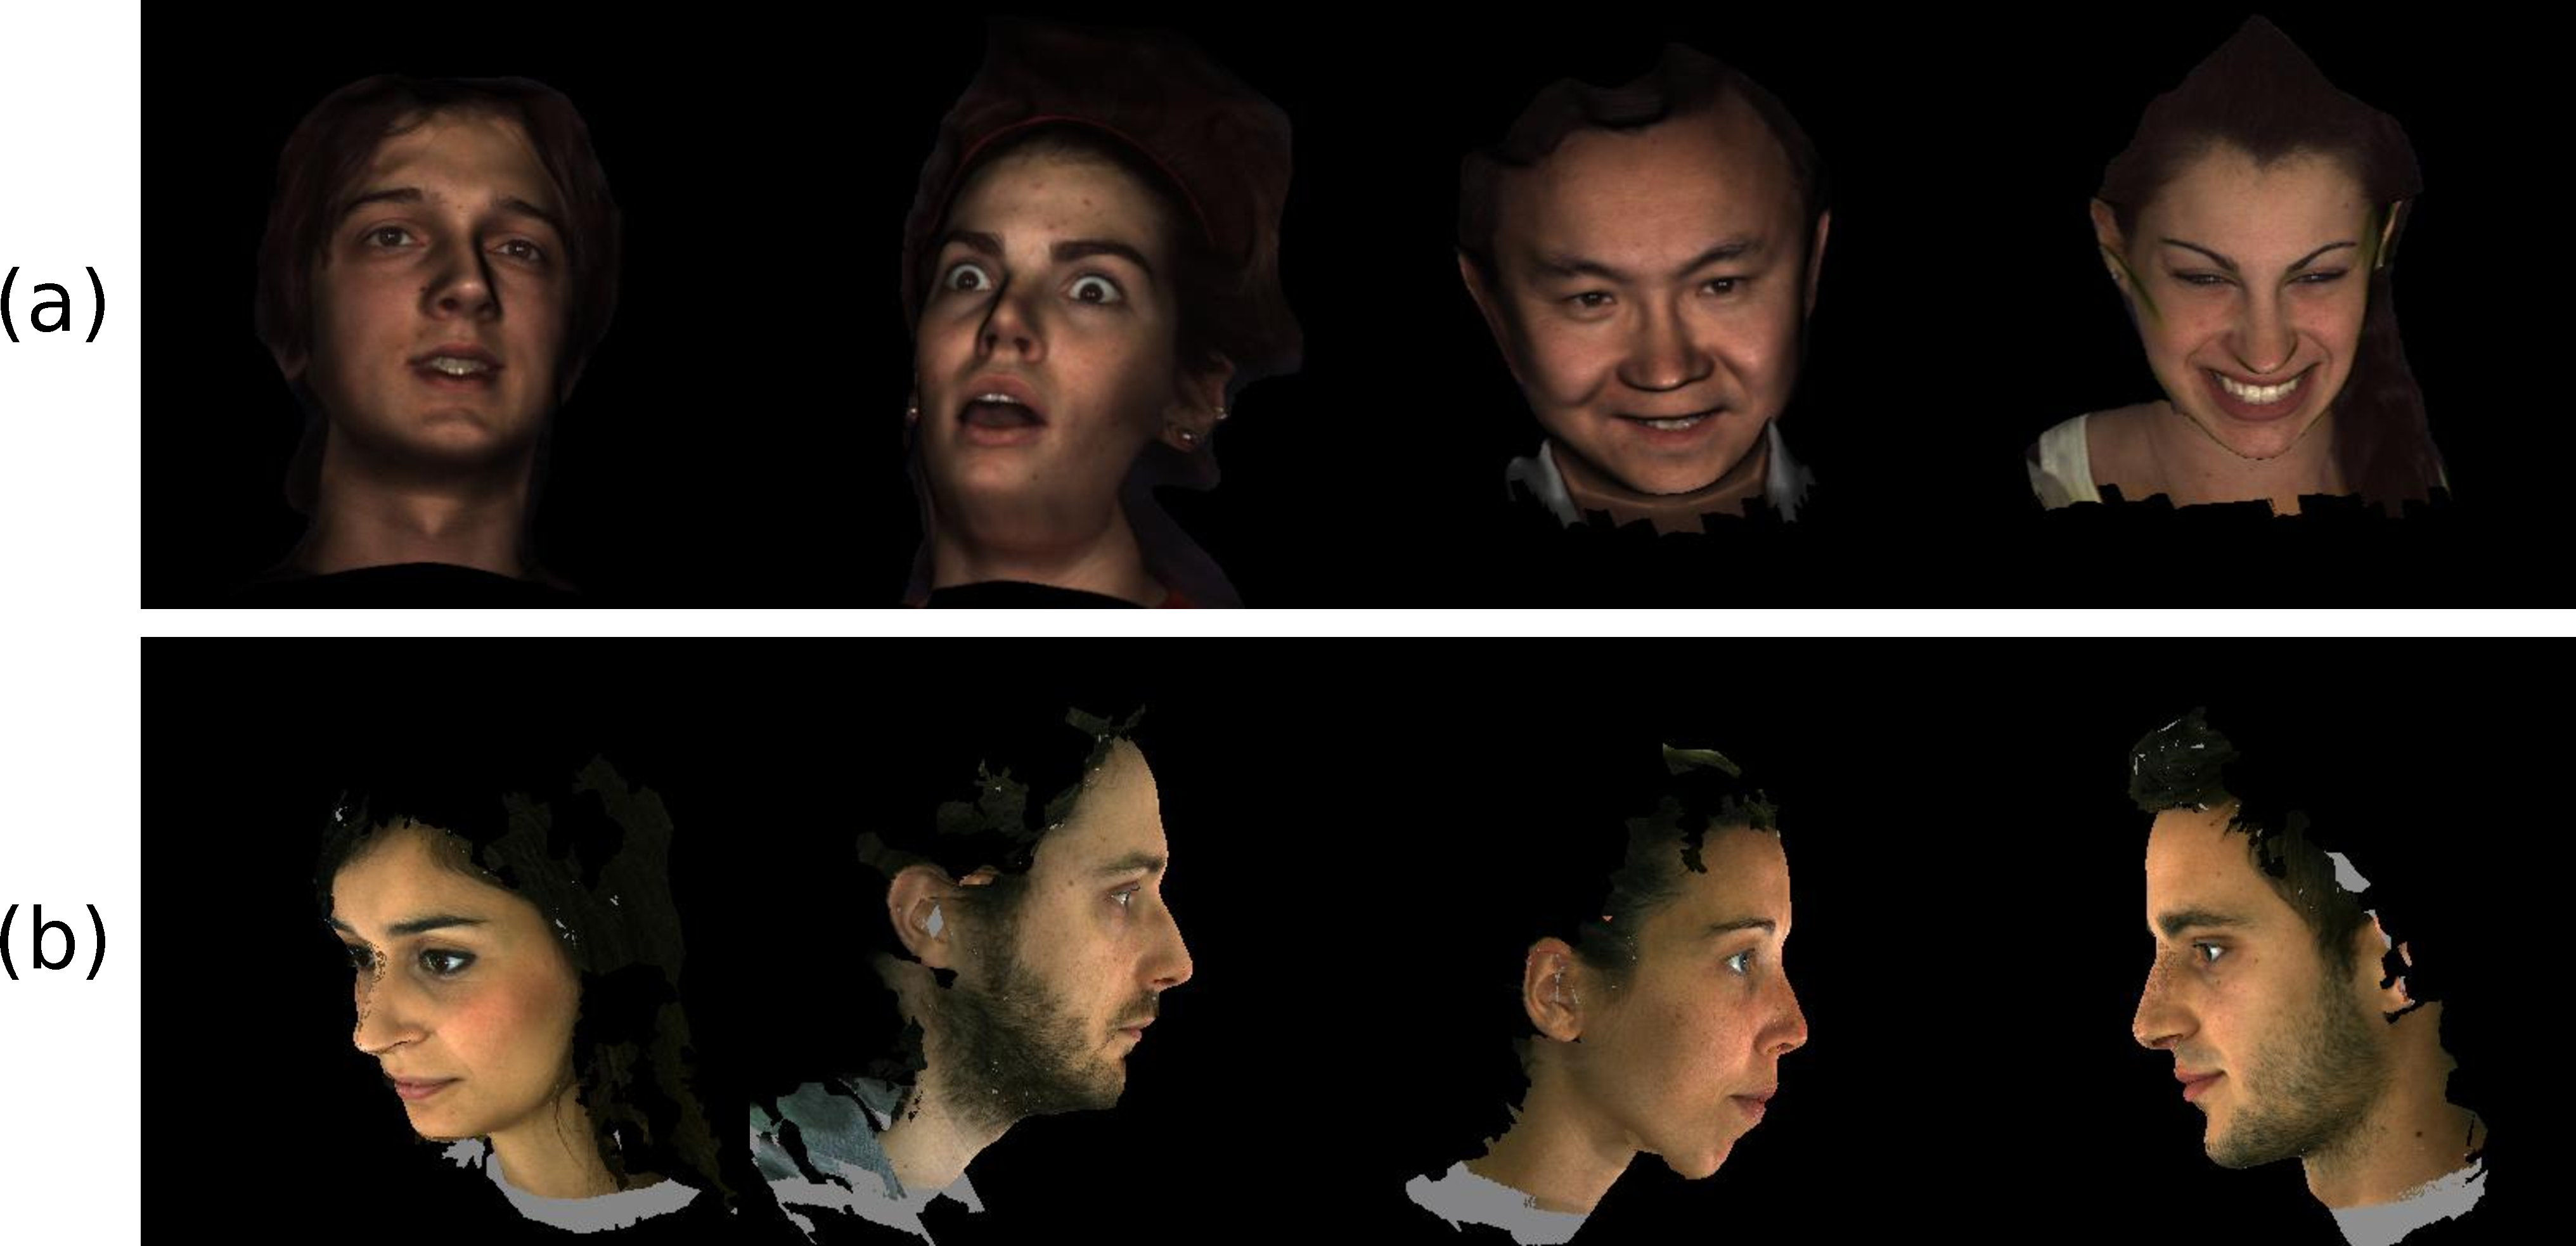
\includegraphics[width=0.9\linewidth]{img/rendering_examples.pdf}
  \caption[Example BU-4DFE and Florence renderings]{Example renderings
    from the BU-4DFE \textbf{(a)} and Florence \textbf{(b)}.}
  \label{fig:example_renderings}
\end{figure}

\subsection{Evaluation metric} To measure the accuracy of reconstruction for
each face, we used the Normalised Mean Error (NME) defined as the
average per vertex Euclidean distance between the estimated and ground
truth reconstruction normalised by the outer 3D interocular distance:

\begin{equation}
  \textrm{NME} = \frac{1}{N} \sum_{k=1}^{N} \frac{||\mathbf{x}_k-\mathbf{y}_{k} ||_{2} }{d}, \label{eq:err}
\end{equation}
\label{eq:3d_nme}
where $N$ is the number of vertices per facial mesh, $d$ is the 3D
outer interocular distance and $\mathbf{x}_k$,$\mathbf{y}_k$ are
vertices of the grouthtruth and predicted meshes. This outer
interocular distance is the distance between the two lateral canthus,
which is the most outer part of the eye. As this is in 3D, the
distance remains fixed even when the face is rotated. The error is
calculated on the face region only on approximately 19,000 vertices
per facial mesh. Notice that when there is no point correspondence
between the ground truth and the estimated mesh, ICP was used but only
to establish the correspondence, i.e. the rigid alignment was not
used. If the rigid alignment is used, we found that, for all methods,
the error decreases but it turns out that the relative difference in
performance remains the same. For completeness, we included these
results in Section~\ref{sec:faceicpres}.


\subsection{Evaluation}

We performed cross-database experiments only, on 3 different
databases, namely AFLW2000-3D, BU-4DFE, and Florence reporting the
performance of all the proposed networks (\textit{VRN}, \textit{VRN -
  Multitask} and \textit{VRN - Guided}) along with the performance of
two state-of-the-art methods, namely 3DDFA \cite{zhu2016face} and EOS
\cite{huber2016multiresolution}. Both methods perform 3DMM
fitting (3DDFA uses a CNN), a process completely bypassed by \textit{VRN}.


% Don't really think this figure demonstrates what we want it to.
% \begin{figure}
%   \centering
%   \begin{tabular}{m{3cm}m{11cm}}
%     Image        & 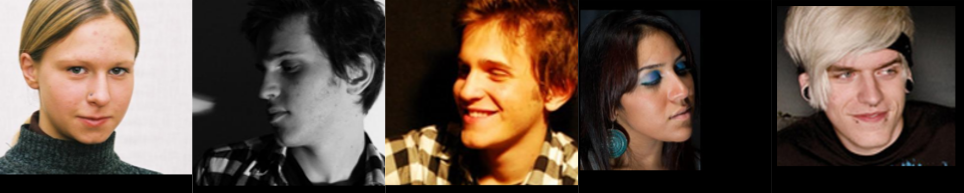
\includegraphics[width=11cm]{img/comparison_r1.png} \\
%     VRN          & 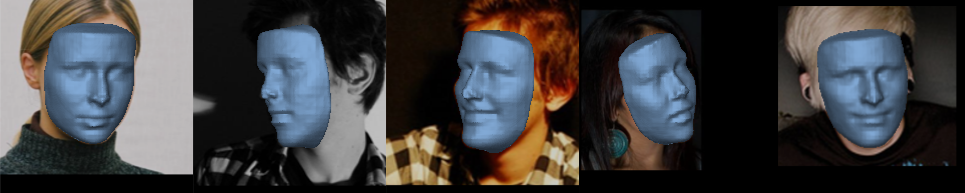
\includegraphics[width=11cm]{img/comparison_r3.png} \\
%     VRN - Guided & 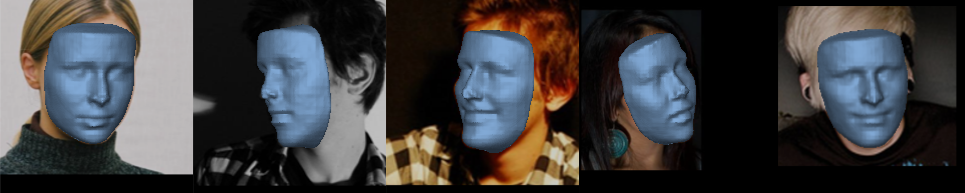
\includegraphics[width=11cm]{img/comparison_r3.png} \\
%   \end{tabular}
% \end{figure}

Our results can be found in Table~\ref{tab:overview} and
Figures~\ref{roc:aflw2000},~\ref{roc:bu4dfe} and~\ref{roc:florence}.
Visual results of the proposed \textit{VRN - Guided} on some very
challenging images from AFLW2000-3D can be seen in
Figure~\ref{fig:aflw2000res}. We show some failure cases in
Figure~\ref{fig:facefailure} where the images are very different to
what has been seen during training time. Finally, we show some example
results from some frames in the 300-VW~\cite{sagonas2013300} video
dataset in Figure~\ref{fig:face300vw}. From all of these results, we
can conclude the following:
\begin{enumerate}
\item Volumetric Regression Networks largely outperform 3DDFA and EOS
  on all datasets used for evaluation, statistically significant in
  all cases ($p < 0.01$, paired $t$-test). This verifies that directly
  regressing the 3D facial structure using the volumetric
  representation, is a much easier problem for CNN learning.
\item All VRNs perform well across the whole spectrum of facial poses,
  expressions and occlusions. Also, there are no significant performance
  discrepancies across different datasets (ALFW2000-3D seems to be
  slightly more difficult).
\item The best performing VRN is the one guided by detected landmarks
  (\textit{VRN - Guided}), however at the cost of higher computational
  complexity: \textit{VRN - Guided} uses another stacked hourglass
  network for landmark localization.
\item \textit{VRN - Multitask} does not always perform better than the
  plain VRN (in fact on BU-4DFE it performs worse), not justifying the
  increase of network complexity. The results are not significant on
  any dataset ($p > 0.10$, paired $t$-test).  It seems that it might
  be preferable to train a network to focus on the task in hand.
\end{enumerate}

\noindent Details about our experiments are given in the proceeding subsections.



\begin{figure}
  \centering
  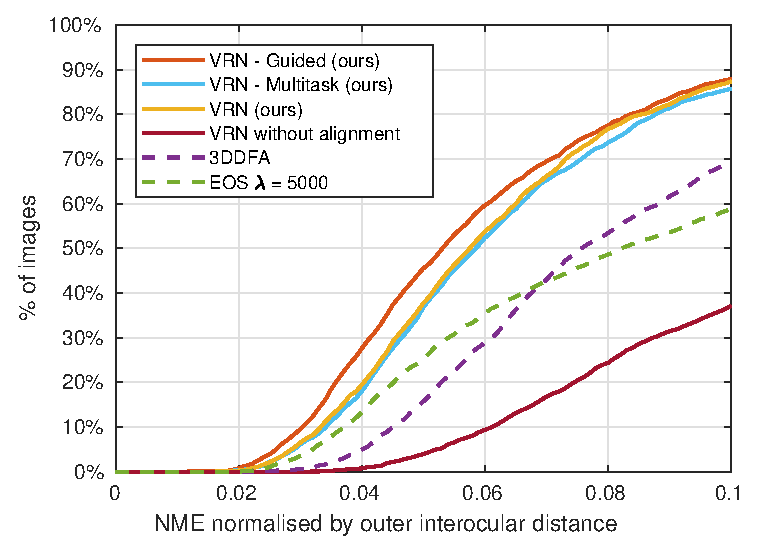
\includegraphics[width=0.75\linewidth]{curves/aflw.eps}
  \caption[NME performance on AFLW2000-3D images]{NME-based
    (Equation~\ref{eq:3d_nme}) performance on in-the-wild ALFW2000-3D
    dataset. The proposed \textit{Volumetric Regression Networks}, and
    EOS and 3DDFA are compared. Please note that ``VRN - without
    allignment'' refers to a VRN where a frontal face is always
    regressed, regardless of input pose, discussed in
    Section~\ref{sec:spatialimportance}.}
  \label{roc:aflw2000}
\end{figure}

\begin{figure}
  \centering
  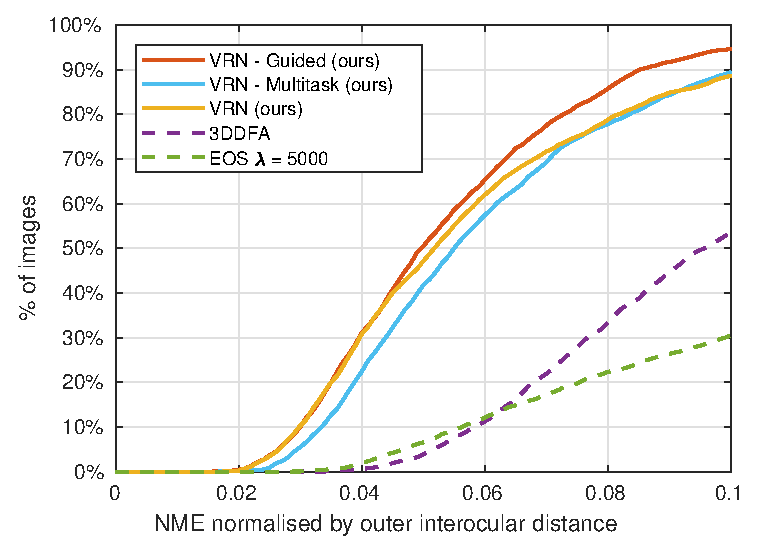
\includegraphics[width=0.75\linewidth]{curves/bu4dfe.eps}
  \caption[NME performance on BU-4DFE renderings]{NME-based
    (Equation~\ref{eq:3d_nme}) performance on renderings from
    BU-4DFE. The proposed \textit{Volumetric Regression Networks}, and
    EOS and 3DDFA are compared.}
  \label{roc:bu4dfe}
\end{figure}

\begin{figure}
  \centering
  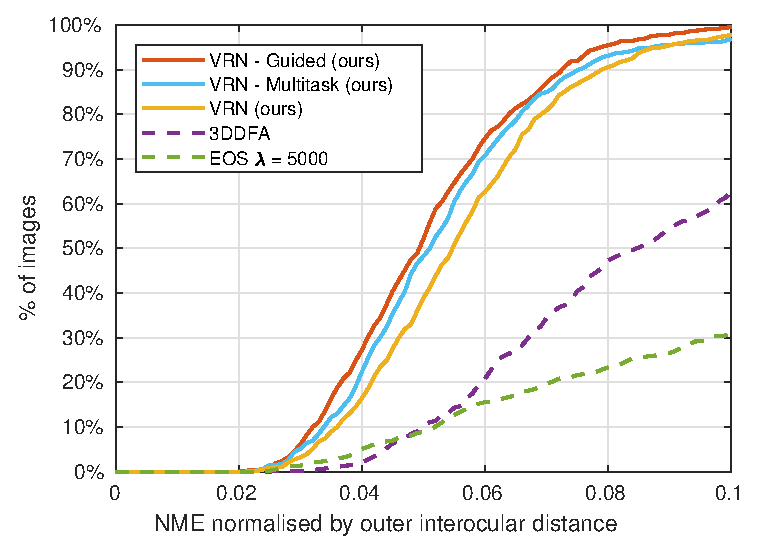
\includegraphics[width=0.75\linewidth]{curves/florence.eps}
  \caption[NME performance on Florence renderings]{NME-based
    (Equation~\ref{eq:3d_nme}) performance on our large pose
    renderings of the Florence dataset. The proposed
    \textit{Volumetric Regression Networks}, and EOS and 3DDFA are
    compared.}
  \label{roc:florence}
\end{figure}




\begin{figure}
  \centering
  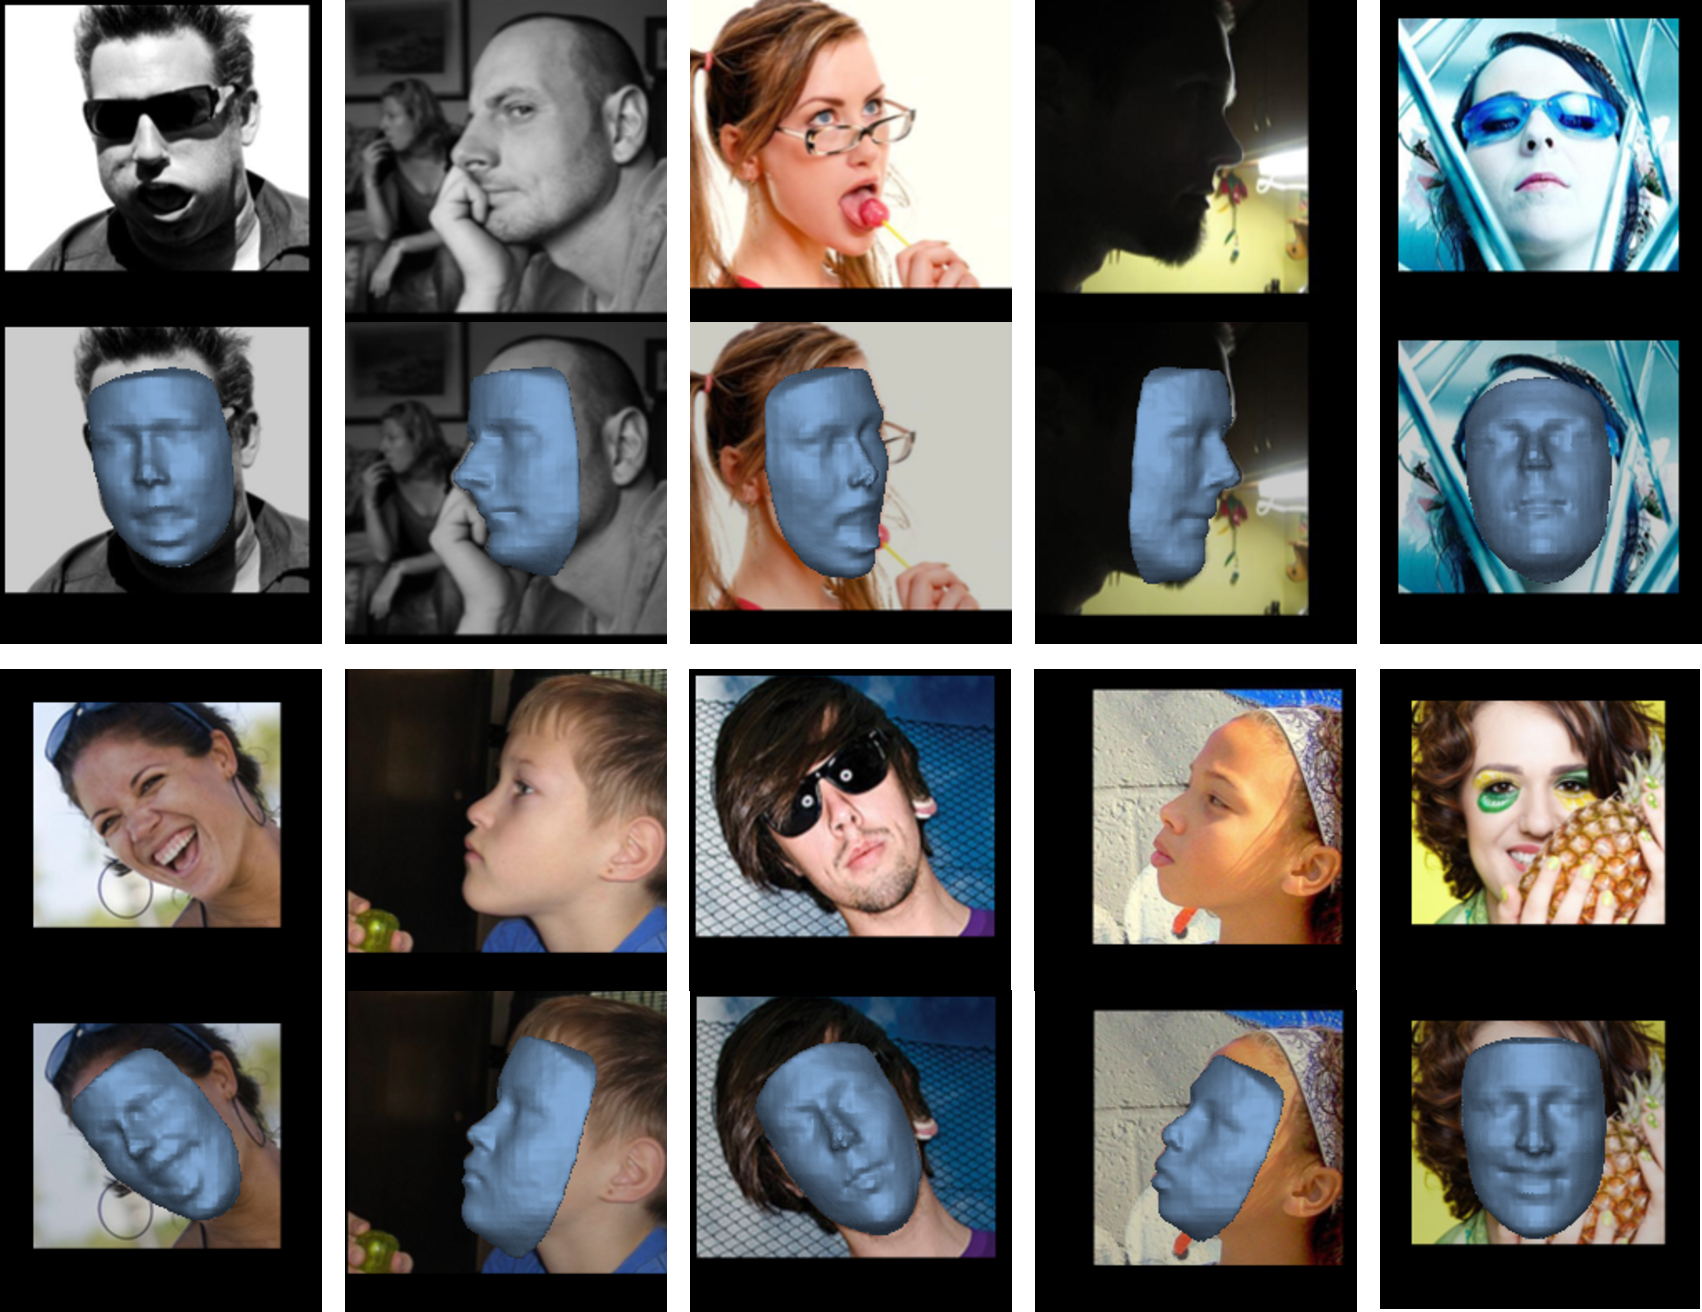
\includegraphics[width=0.7\linewidth]{img/aflw2000res.pdf}
  \caption[Visual results on AFLW2000-3D dataset]{Some visual results
    from the AFLW2000-3D dataset generated using our \textit{VRN -
      Guided} method.}
  \label{fig:aflw2000res}
  \vspace{-4mm}
\end{figure}


\begin{figure}
  \centering
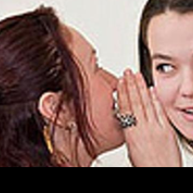
\includegraphics[width=3.4cm]{img/failures/image00400_img.png}
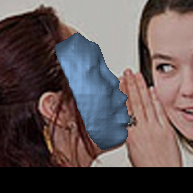
\includegraphics[width=3.4cm]{img/failures/image00400_vol.png} \hspace{2mm}
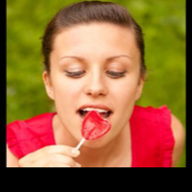
\includegraphics[width=3.4cm]{img/failures/image00782_img.png}
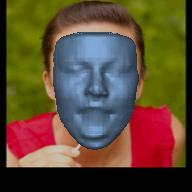
\includegraphics[width=3.4cm]{img/failures/image00782_vol.png}  \\ [0.5mm]
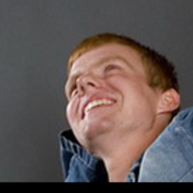
\includegraphics[width=3.4cm]{img/failures/image00795_img.png}
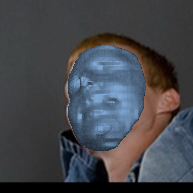
\includegraphics[width=3.4cm]{img/failures/image00795_vol.png} \hspace{2mm}
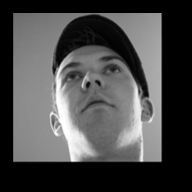
\includegraphics[width=3.4cm]{img/failures/image01038_img.png}
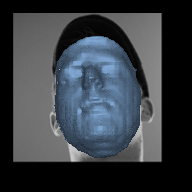
\includegraphics[width=3.4cm]{img/failures/image01038_vol.png}  \\ [0.5mm]
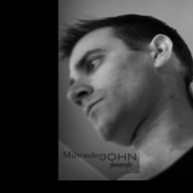
\includegraphics[width=3.4cm]{img/failures/image01624_img.png}
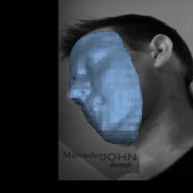
\includegraphics[width=3.4cm]{img/failures/image01624_vol.png} \hspace{2mm}
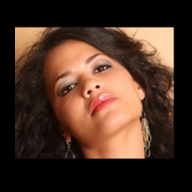
\includegraphics[width=3.4cm]{img/failures/image02026_img.png}
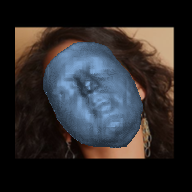
\includegraphics[width=3.4cm]{img/failures/image02026_vol.png}
\caption[Some very difficult failure cases]{Some failure cases on
  AFLW2000 from our \textit{VRN - Guided} network. In general, these
  images are poses which are not seen in the training set.}
\label{fig:facefailure}
\end{figure}

\begin{figure}
  \centering
  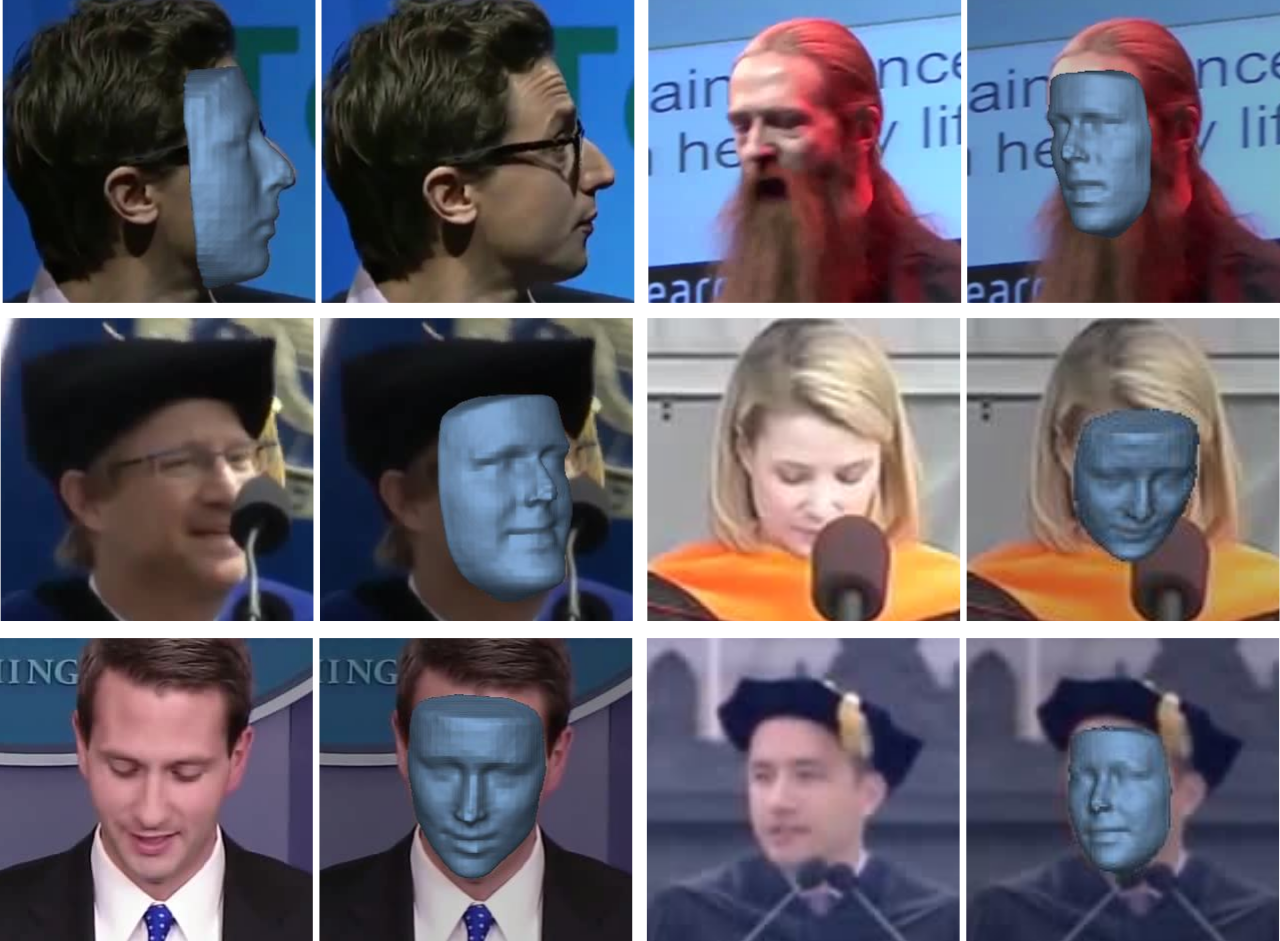
\includegraphics[width=0.9\linewidth]{img/300vw.png}
  \caption[Visual results on the 300VW dataset]{Some example results
    from frames of the 300VW dataset.}
  \label{fig:face300vw}
\end{figure}


\subsubsection{Comparison with state-of-the-art}
We compared against state-of-the-art 3D reconstruction methods for
which code is publicly available. These include the very recent
methods of 3DDFA~\cite{zhu2016face}, and
EOS~\cite{huber2016multiresolution}. For EOS we used a large
regularisation parameter $\lambda = 5000$ which we found to offer the
best performance for most images. The method uses 2D landmarks as
input, so for the sake of a fair comparison a stacked hourglass for 2D
landmark detection was trained for this purpose. Our tests were
performed using v0.12 of EOS.


\subsection{Results with ICP Alignment}
\label{sec:faceicpres}

We present results where ICP has been used not only to find the
correspondence between the groundtruth and predicted vertices, but
also to remove the rigid transformation between them. ICP was applied
after the surface extraction was used to create the mesh. We find that
this offers a marginal improvement to all methods. However, the
relative performance remains mostly the same between each
method. Results on AFLW2000~\cite{zhu2016face},
BU4DFE~\cite{yin2008high} and Florence~\cite{masi2d3dFaceData} can be
seen in Figs.~\ref{roc:aflw2000icp},~\ref{roc:bu4dfeicp}
and~\ref{roc:florenceicp} respectively. Numeric results can be found
in Table~\ref{tab:overviewicp}.

\begin{table}
  \caption[Numerical performance of 3D face reconstruction with
  ICP]{Reconstruction accuracy on AFLW2000-3D, BU4DFE and Florence in
    terms of NME (Equation~\ref{eq:3d_nme}) where ICP has been used to
    remove the rigid transformation. Lower is better. }
  \label{tab:overviewicp}
  \centering\vspace{1mm}
  \small
\begin{tabular}{|l||c|c|c|}
  \hline
  \textbf{Method}   & \textbf{AFLW2000} & \textbf{BU4DFE} & \textbf{Florence} \\
  \hline\hline
  VRN               & 0.0605 & 0.0514 & 0.0470   \\
  VRN - Multitask   &   0.0625    & 0.0533     & 0.0439        \\
  VRN - Guided      & \textbf{0.0543} & \textbf{0.0471} & \textbf{0.0429}   \\

\hline
  3DDFA~\cite{zhu2016face}             & 0.1012 & 0.1144 & 0.0784   \\
  EOS~\cite{huber2016multiresolution}  & 0.0890 & 0.1456 & 0.1200   \\
  \hline
\end{tabular}
\end{table}

\begin{figure}
  \centering
  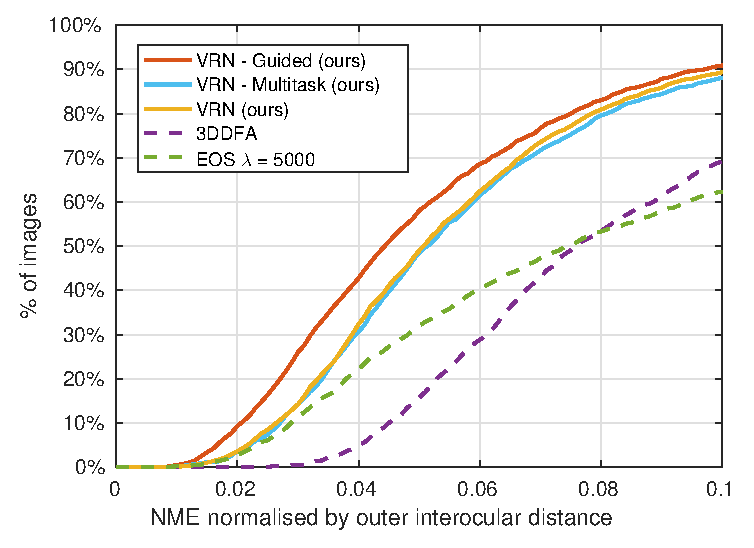
\includegraphics[width=0.75\linewidth]{curves-icp/aflw.eps}
  \caption[NME performance on AFLW2000-3D with ICP
  Alignment]{NME-based (Equation~\ref{eq:3d_nme}) performance on the
    in-the-wild AFLW2000-3D dataset, where ICP has been used to remove
    the rigid transformation. The proposed \textit{Volumetric
      Regression Networks}, and EOS and 3DDFA are compared.}
  \label{roc:aflw2000icp}
\end{figure}

\begin{figure}
  \centering
  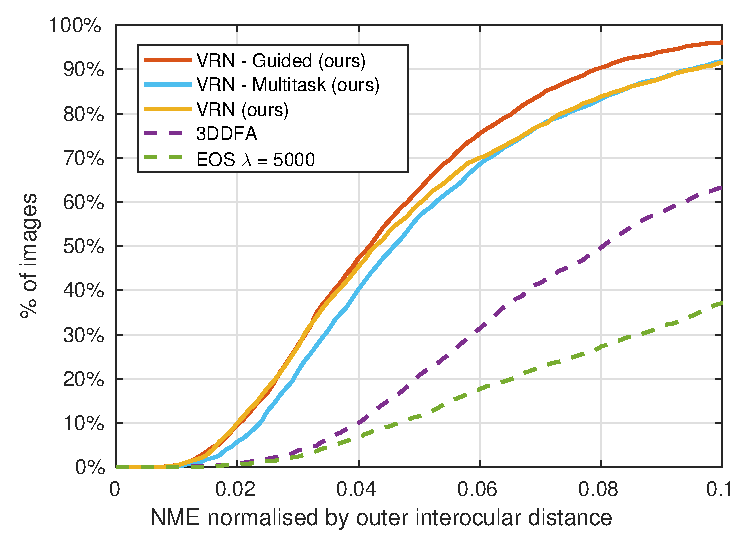
\includegraphics[width=0.75\linewidth]{curves-icp/bu4dfe.eps}
  \caption[NME performance on BU4DFE with ICP Alignment]{NME-based
    (Equation~\ref{eq:3d_nme}) performance on our large pose and
    expression renderings of the BU4DFE dataset, where ICP has been
    used to remove the rigid transformation. The proposed
    \textit{Volumetric Regression Networks}, and EOS and 3DDFA are
    compared.}
  \label{roc:bu4dfeicp}
\end{figure}

\begin{figure}
  \centering
  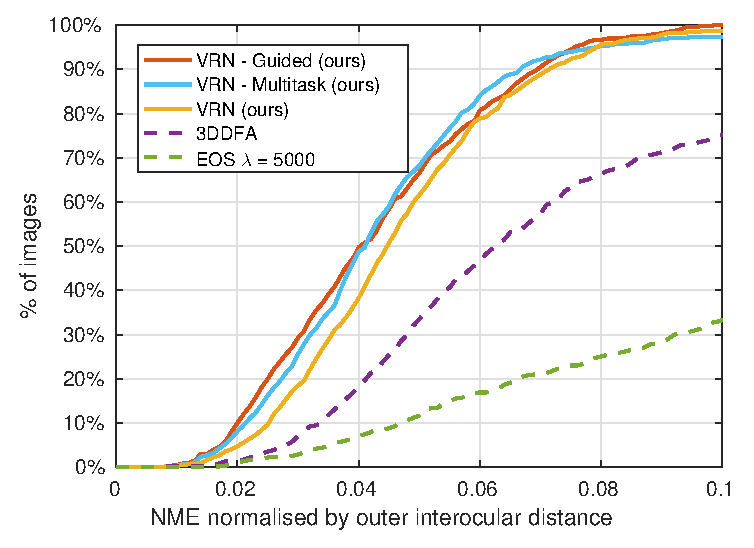
\includegraphics[width=0.75\linewidth]{curves-icp/florence.eps}
  \caption[NME performance on Florence with ICP Alignment]{NME-based
    (Equation~\ref{eq:3d_nme}) performance on our large pose
    renderings of the Florence dataset, where ICP has been used to
    remove the rigid transformation. The proposed \textit{Volumetric
      Regression Networks}, and EOS and 3DDFA are compared.}
  \label{roc:florenceicp}
\end{figure}


\section{Importance of spatial alignment}
\label{sec:spatialimportance}

Our approach to 3D face reconstruction preserves the spatial alignment
between input and output. That is to say that the regressed 3D
geometry should be capable of segmenting the input face from the
background, given a 2D orthographic projection of the volume. A 3D
reconstruction method is described in~\cite{choy20163d} which accepts
as input one or more images, and as output, produces a small 3D volume
of $32 \times 32 \times 32$ using an LSTM. In an attempt to explore
what the repercussions of ignoring spatial alignment are, we trained a
variant of \textit{VRN} which regresses a frontal version of the face,
i.e. a face of fixed orientation, regardless of input pose, as
in~\cite{choy20163d}. We call this fixed-pose variant of our method
\textit{VRN - without alignment}. We also attempted to train a network
using the code from~\cite{choy20163d} on downsampled versions of our
volumes. Unfortunately we were unable to get the network to learn
anything and found that the loss would now reduce.

Although \textit{VRN - without alignment} produces a reasonable face,
it captures only a diminished expression. The shape for all faces
appears to remain almost identical across all images. This is very
noticeable in Figure~\ref{fig:frontal_visual}. Numeric comparison is
shown in Figure~\ref{roc:aflw2000}, as \textit{VRN - without
  alignment}. We believe that this further confirms that
\textbf{spatial alignment is of paramount importance} when performing
3D reconstruction in this way.

\begin{figure}
  \centering
  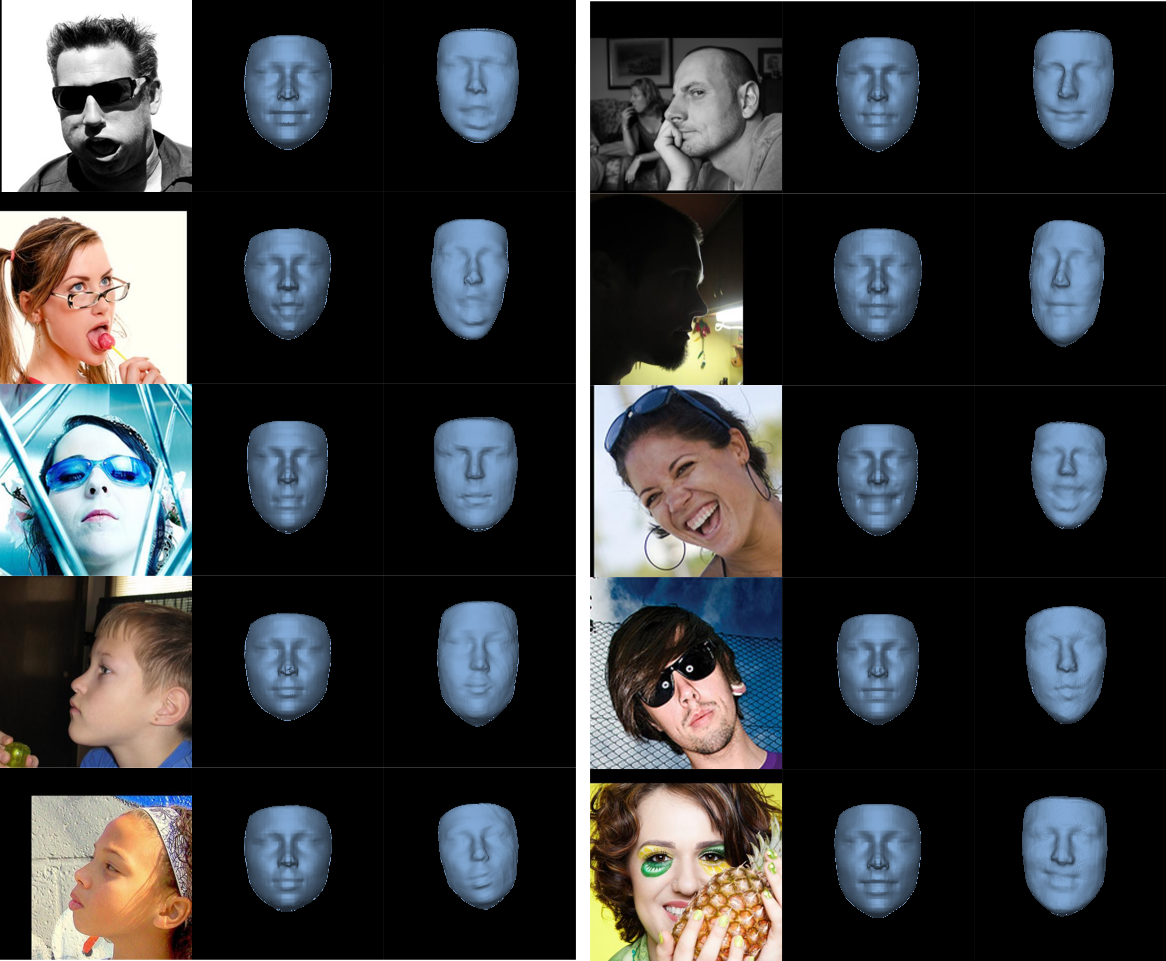
\includegraphics[width=0.7\linewidth]{img/frontal.png}
  \caption[Visual results when spatial alignment is ignored]{Result from
    \textit{VRN without alignment} (second columns), and a frontalised
    output from \textit{VRN - Guided} (third columns).}
  \label{fig:frontal_visual}
\end{figure}

\section{Ablation studies}
\label{chapter:face:sec:ablation}

In this section, we report the results of experiments aiming to shed
further light into the performance of the proposed networks. For all
experiments reported, we used the best performing \textit{VRN -
  Guided}.

\subsection{Effect of pose}

To measure the influence of pose on the reconstruction error, we
measured the NME (Equation~\ref{eq:3d_nme}) for different amounts of
yaw using all of our Florence~\cite{masi2d3dFaceData}
renderings. These were rendered at $\{-80, -40, 0, 40, 80\}$ degrees
of yaw for each of $\{-5, 0, 5\}$ degrees of pitch, for all 50
subjects in Florence. As shown in Figure~\ref{fig:effect_pose}, the
performance of our method decreases as the pose increases. This is to
be expected, due to less of the face being visible which makes
evaluation for the invisible part difficult. We believe that our error
is still very low considering the magnitude of these poses.



\subsection{Effect of expression} Certain expressions are usually
considered harder to accurately reproduce in 3D face reconstruction.
To measure the effect of facial expressions on performance, we
rendered frontal images in difference expressions from BU-4DFE (since
Florence only exhibits a neutral expression) and measured the
performance for each expression. We show the six acted facial
expressions which are available in BU-4DFE in
Figure~\ref{fig:bu4dfe_expressions}. These expressions are available
for all participants, of which there are 102. This kind of extreme
acted facial expressions generally do not occur in the training set,
yet as shown in Figure~\ref{fig:effect_expression}, the performance
variation across different expressions is quite minor.

\begin{figure}
  \centering
  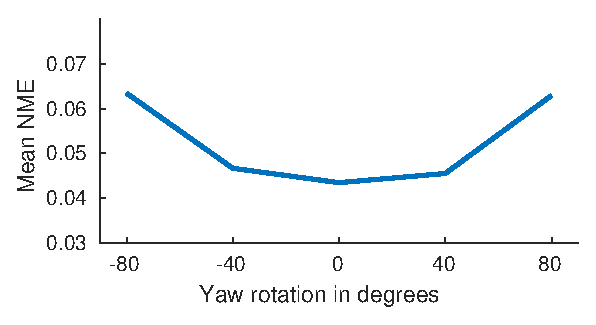
\includegraphics[width=0.6\linewidth]{curves/ablation_pose.eps}
  \caption[Effect of pose]{The effect of pose on reconstruction
    accuracy in terms of NME (Equation~\ref{eq:3d_nme}) on the
    Florence dataset. The \textit{VRN - Guided} network was used.}
  \label{fig:effect_pose}
\end{figure}

\begin{figure}
  \centering
  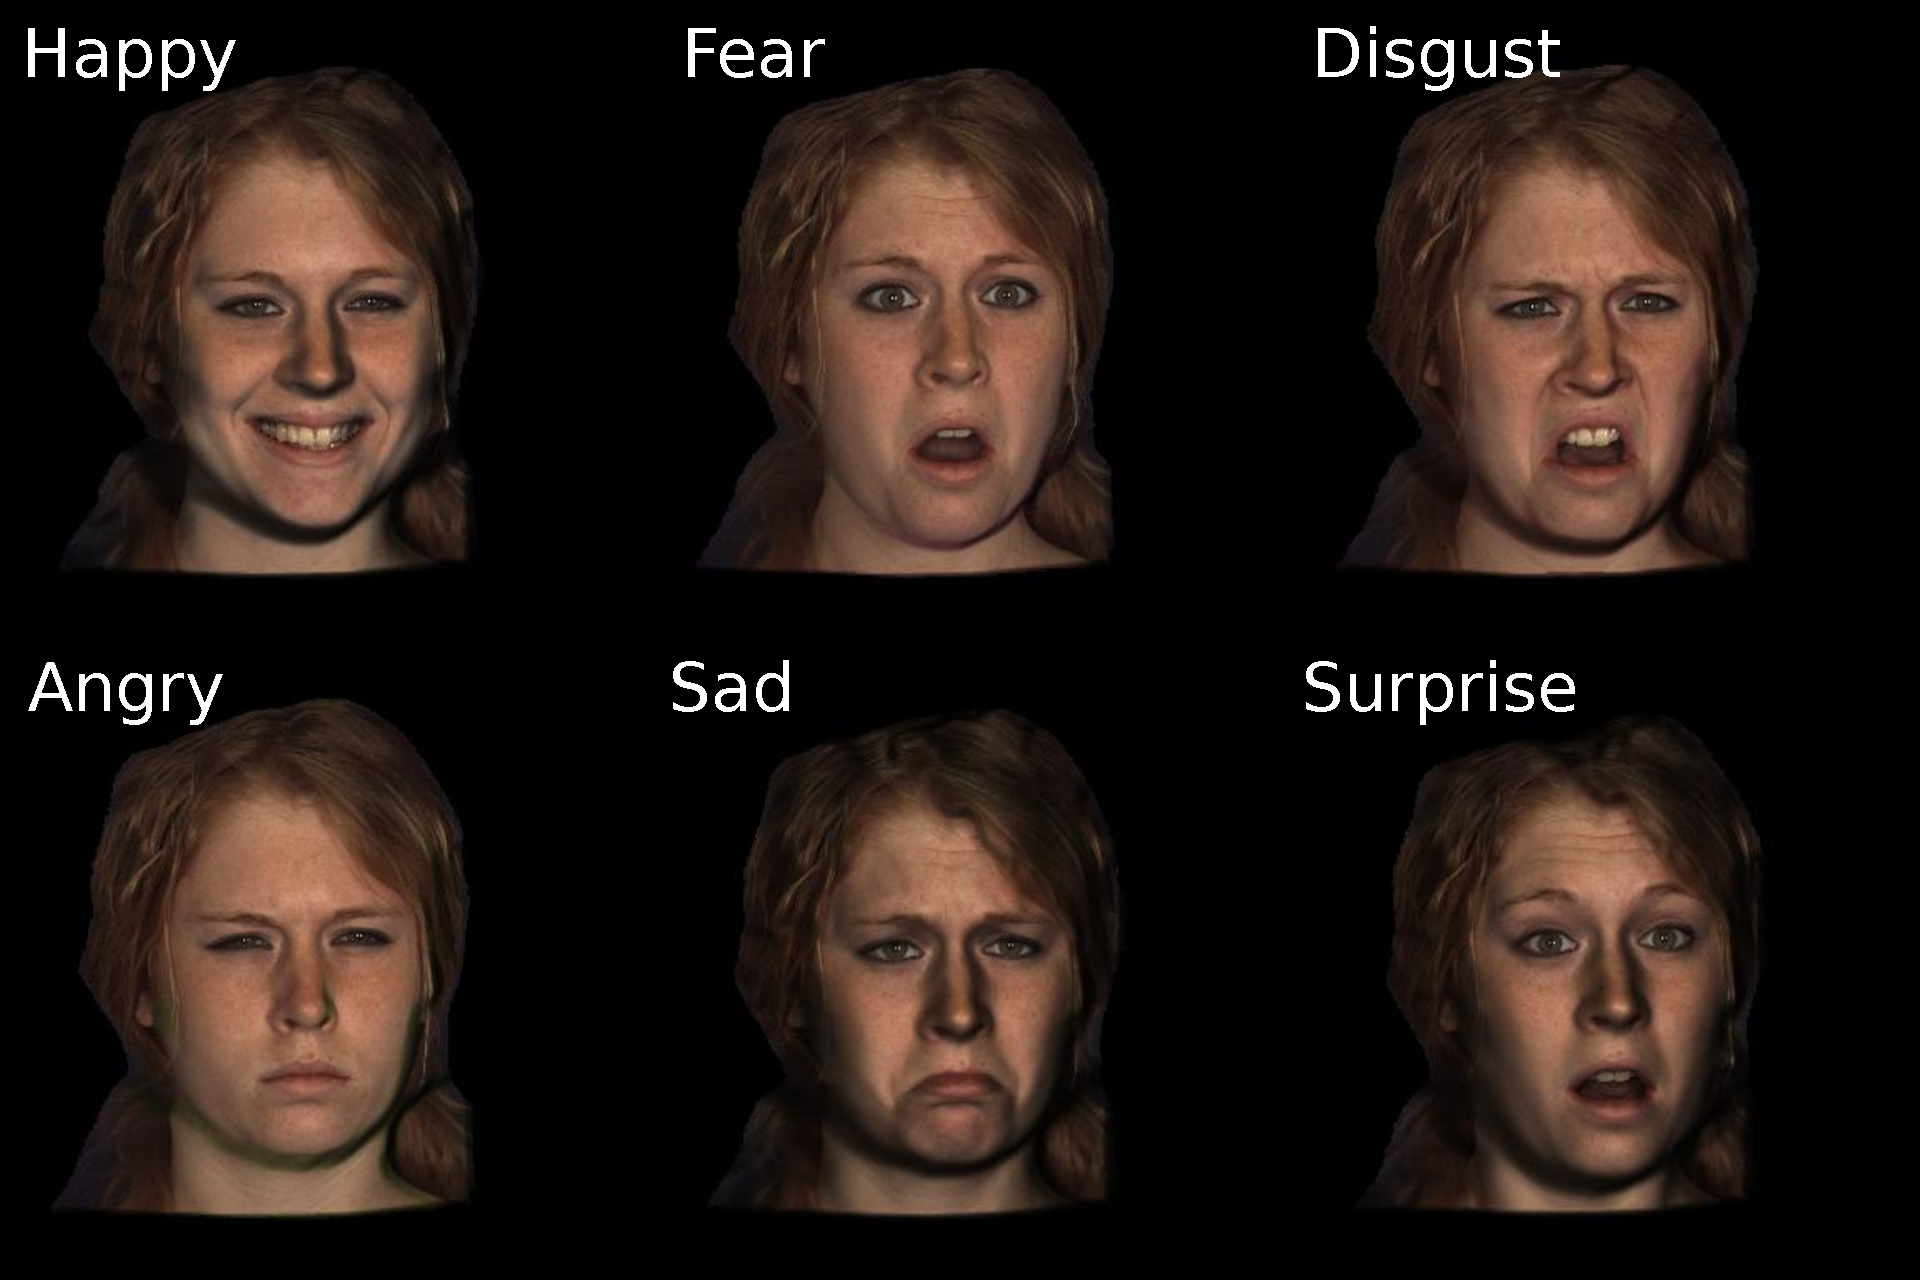
\includegraphics[width=0.8\linewidth]{img/bu4dfe_expressions.pdf}
  \caption[The six facial expressions available in the BU-4DFE
  dataset]{The six facial expressions available in the BU-4DFE
    dataset~\cite{yin2008high}, rendered for the same participant.}
  \label{fig:bu4dfe_expressions}
\end{figure}

\begin{figure}
  \centering
  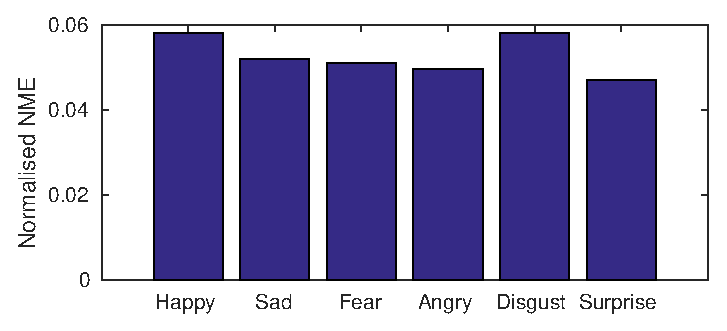
\includegraphics[width=0.7\linewidth]{curves/ablation_expression.eps}
  \caption[Effect of facial expressions]{The effect of facial
    expression on reconstruction accuracy in terms of NME
    (Equation~\ref{eq:3d_nme}) on the BU-4DFE dataset. The \textit{VRN
      - Guided} network was used.}
  \label{fig:effect_expression}
\end{figure}

\subsection{Effect of Gaussian size for guidance} We trained a
\textit{VRN - Guided}, however, this time, the facial landmark
detector network of the \textit{VRN - Guided} regresses larger
Gaussians ($\sigma = 2$ as opposed to the normal $\sigma = 1$). The
performance of the 3D reconstruction dropped by a negligible amount,
suggesting that as long as the Gaussians are of a sensible size,
guidance will always help.

\section{Architectural Experiments}
\label{sec:arcexp}

In this section we explore several variations and modifications to the
\textit{VRN - Guided} method, which may improve or impede
performance. We provide an overview of experiments along with NME
(Equation~\ref{eq:3d_nme}) in Table~\ref{tab:arcexpoverview}.

\begin{table*}
  \caption[Overview of architectural experiments]{An overview of the
    architectural experiments conducted. \textbf{Feats} refers to the
    number of features per convolution layer. Similarly,
    \textbf{VFeats} refers to the number of volumetric features per
    volumetric convolution (in most cases this has no value as the
    majority of the networks used in our experiments are 2D
    only). \textbf{Mod} refers to the number of Residual modules used
    sequentially in any one place of the hourglass. \textbf{Stack}
    refers to the number of hourglass networks in a single stack. The
    right most column points to the relevant section of the
    chapter. We also show the mean Normalised Mean Error (NME,
    Equation\ref{eq:3d_nme}) for all images of the AFLW2000 dataset in
    column \textbf{nNME}.}
  \label{tab:arcexpoverview}
  \centering
  \small
  \begin{tabular}{|r|| c|c|c|c || c || c|l|}
    \hline
    \textbf{Name} & \textbf{Feats} & \textbf{VFeats} & \textbf{Mod} & \textbf{Stack} &  \textbf{Para} & \textbf{mNME} & \textbf{Sec.} \\
    \hline\hline
    VRN - Guided             & 256    & ---     & 4        & 2  & $2.5\times 10^7$    & 0.0637 &   \\
    \hline
    Intermediate Supervis.   & 256    & ---     & 4        & 2  & $2.5\times 10^7$    & 0.0630 & \ref{sec:arc_intersup}  \\
    \hline
    Hourglass                & 256    & ---     & 8        & 1  & $2.5\times 10^7$    & 0.0621 &   \\
    Three Hourglass          & 256    & ---     & 3        & 3  & $2.8\times 10^7$    & 0.0632 & \ref{sec:arc_secvsmod}  \\
    Four Hourglass           & 256    & ---     & 2        & 4  & $2.7\times 10^7$    & 0.0639 &   \\
    \hline
    Hourglass Heavy          & 384    & ---     & 8        & 1  & $5.3\times 10^7$    & 0.0627 &   \\
    Hourglass Light          & 128    & ---     & 8        & 1  & $6.3\times 10^6$    & 0.0633 & \ref{sec:arc_params}  \\
    Hourglass Lighter        & 64     & ---     & 8        & 1  & $1.8\times 10^6$    & 0.0661 &   \\
    \hline
    Volumetric VRN           & 128    & 32      & 2        & 2  & $7.7\times 10^5$    & 0.0697 & \ref{sec:arc_volumetric} \\
    \hline
  \end{tabular}
\end{table*}

\subsection{On intermediate supervision}
\label{sec:arc_intersup}

As described in the original stacked hourglass
paper~\cite{newell2016stacked}, intermediate supervision is typically
used providing significant boost in performance. However, it was not
implemented for the basic \textit{VRN} or \textit{VRN - Guided}
networks. As an attempt to boost performance, we have trained an
identical network to \textit{VRN - Guided}, except with a supervising
loss after the first hourglass network. A very minor performance
improvement can be observed, as shown in
Table~\ref{tab:arcexpoverview}. Additionally, the corresponding curve
can be seen in Figure~\ref{fig:additionalexp}. We conclude that
intermediate supervision is not necessary to achieve high performance
for our 3D reconstruction experiment.

%It is possible that in
%\cite{newell2016stacked}, higher performance were observed by using
%intermediate supervision, simply because there were many more
%hourglasses in a stack.


\subsection{On increasing the number of stacks vs the number of modules}
\label{sec:arc_secvsmod}

Given a fixed computational budget one has two options when
implementing a Volumetric Regression Network: to increase the number
of stacks while decreasing the number of modules or vice versa.  An
interesting question which has now been answered yet is whether it is
better to have more stacked hourglasses or more modules per
hourglass. In this section, we attempt to quantify any performance
variation, at least for the task of 3D face reconstruction using
volumetric regression while keeping the number of parameters
approximately the same.

We evaluate three additional networks, each with different number of
hourglasses and modules, such that the total number of parameters
remains very similar. These results are shown in detail in
Table~\ref{tab:arcexpoverview} as One, Three or Four Hourglass. The
first of these additional networks consists of only one hourglass
network and eight modules. Interestingly, this performs the best out
of the three, suggesting that for this particular problem, perhaps it
is more optimal to increase the number of modules over the number of
hourglasses. This may also be observed from a single hourglass
outperforming \textit{VRN - Guided}, which again, may be due to higher
performance gains from more modules over stacked hourglasses.However,
it can also be observed that the performance difference between all
networks is very minor, suggesting that for our experiment as long as
the number of parameters remains roughly fixed good performance can be
achieved independently of the exact configuration of the hourglass
network.
%Perhaps our performance bottleneck is not the network but the dataset
%from which we are learning, which may be the case if there exists any
%noise.


\subsection{On varying the network parameters}
\label{sec:arc_params}

Having investigated the importance of network configuration in the
previous section, in this section we keep the architecture fixed and
instead vary the number of network parameters to quantify the the
performance impact. Hence, in this section we explore the influence of
number of parameters, and whether the performance will continue to
increase with the number of parameters, or the same performance can be
achieved with fewer parameters. If performance saturation has
occurred, the dataset has likely become the limiting factor, likely
due to variance in the training set, suggesting that it may be
possible to achieve a similar level of performance with fewer
parameters.

We explore 3 variants of the VRN, corresponding to different number of
parameters, namely \textit{Heavy}, \textit{Light} and
\textit{Lighter}. Their exact number of parameters and performance is
shown in Table~\ref{tab:arcexpoverview}. It can be observed that the
performance difference between \textit{Heavy} and \textit{Light} are
very minor. However, \textit{Lighter} resulted in a significant drop
in performance. With this information we can hypothesise that the
optimal number of parameters is the one corresponding to the
\textit{Light} network. We show a visual comparison between these
three networks in Figure~\ref{fig:heavy-light-lighter}: the visual
performance of the \textit{Lighter} network is clearly worse - the
surface is not as smooth and the facial expression is not captured as
clearly as in both \textit{Heavy} and \textit{Light}.

\subsection{A Volumetric Implementation}
\label{sec:arc_volumetric}

One of the main contributions of this chapter is to show that good
performance for 3D face reconstruction can be achieved even when 2D
spatial convolutions are used.  However, one might wonder why we
decided to use 2D convolutions for a 3D (volumetric) regression
task. The short answer is that training a 3D CNN is difficult and
highly resource intensive. Firstly, the activations are much larger,
consuming more memory leaving less space for parameters. Secondly, the
complexity of volumetric convolution is much higher than that of
standard spatial convolution, hence the time required to train such a
network is far greater, despite the potential for fewer parameters.

For completeness, we have trained a fully volumetric version of VRN
where we attempt to match this time the complexity in theoretical
floating point operations (FLOPS) for a single forward pass (as
opposed to matching the number of parameters) with that of a standard
VRN. We use theoretical FLOPS, as opposed to actual or raw number of
FLOPS, as frameworks such as CuDNN make numerous optimisations, which
often result in fewer operations. Unfortunately, this resulted in
having only 32 features per volumetric convolution.

Despite containing far fewer parameters than the standard VRN, the
training took over 10 days on two Titan X GPUs and had to be performed
with a batch size of 2. This is significantly slower than training the
standard VRN, which takes approximately 2 days on the same
hardware. We show the NME (Equation~\ref{eq:3d_nme}) for this network in
Table~\ref{tab:arcexpoverview}, along with a curve in
Figure~\ref{fig:additionalexp}. Unsurprisingly, the performance of
this method is quite poor, further illustrating the difficulty in
training 3D CNNs despite the problem being a volumetric one.

\subsection{Architectural Conclusions}
As we have seen from the past few experiments, performance in general
remains very similar despite architectural changes. Only after
reducing the number of parameters significantly were we able observe
any significant change. We conclude that with the guidance from
detected landmarks only, we are almost able to attain the best performance on
these datasets.

\begin{figure}
  \centering
  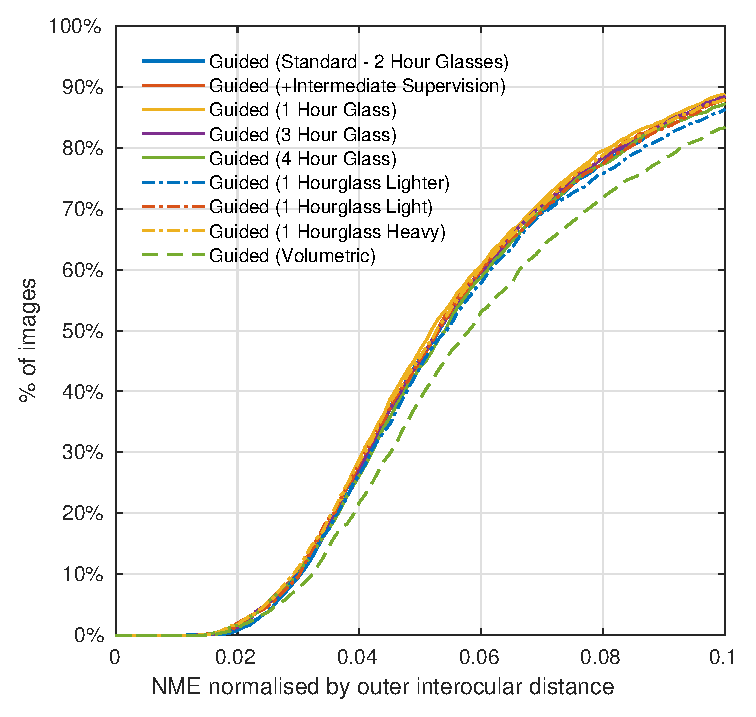
\includegraphics[width=0.75\linewidth]{curves2/aflw.eps}
  \caption[NME performance from architectural experiments]{Results in
    NME (Equation~\ref{eq:3d_nme}) from architectural experiments
    described in Section~\ref{sec:arcexp} on the AFLW2000 dataset,
    showing that in the majority of cases the performance is almost
    the same.}
  \label{fig:additionalexp}
\end{figure}

\begin{figure}
  \centering
  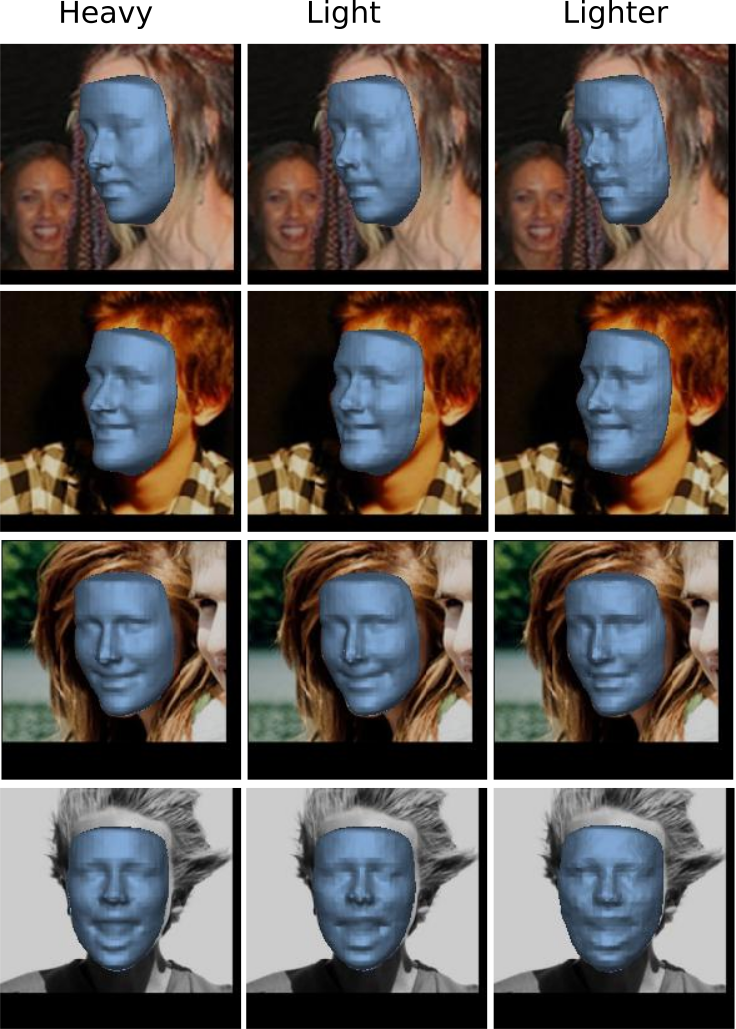
\includegraphics[width=0.75\linewidth]{img/heavy-light-lighter.png}
  \caption[Visual comparison of number of parameters]{A visual
    comparison between the \textit{Heavy}, \textit{Light} and
    \textit{Lighter} methods described in Section~\ref{sec:arc_params}
    on three images from the AFLW2000 dataset.}
  \label{fig:heavy-light-lighter}
\end{figure}



\section{Conclusions}

We proposed a direct approach to 3D facial reconstruction from a
single 2D image using volumetric CNN regression. To this end, we
proposed and exhaustively evaluated three different networks for
volumetric regression, reporting results that show that the proposed
networks perform well for the whole spectrum of facial pose, and can
deal with facial expressions as well as occlusions. We also compared
the performance of our networks against that of recent
state-of-the-art methods based on 3DMM fitting reporting large
performance improvement on three different datasets.  Future work may
include improving detail and establishing a fixed correspondence from
the isosurface of the mesh.


%%% Local Variables:
%%% TeX-master: "../thesis"
%%% End: